\documentclass[officiallayout]{tktla}

\usepackage[utf8]{inputenc}
\usepackage[T1]{fontenc}

\usepackage{graphicx}
\usepackage{url}
\usepackage{longtable}

\usepackage{amsmath}
\usepackage{amssymb}
\usepackage{amsfonts}
\usepackage{amsthm}


\title{Compressed Full-Text Indexes for Highly Repetitive Collections}
\author{Jouni Sirén}
\authorcontact{jouni.siren@cs.helsinki.fi\par
  http://www.cs.helsinki.fi/jouni.siren/}
\pubtime{June}{2012}
\reportno{5}
\isbnpaperback{978-952-10-8051-7}
\isbnpdf{978-952-10-8052-4}
\issn{1238-8645}
\printhouse{Unigrafia}
\pubpages{97 + 63}
\supervisorlist{Veli Mäkinen, University of Helsinki, Finland}
\preexaminera{Kunihiko Sadakane, National Institute of Informatics, Japan}
\preexaminerb{Jorma Tarhio, Aalto University, Finland}
\opponent{Giovanni Manzini, University of Eastern Piedmont, Italy}
\custos{Veli Mäkinen, University of Helsinki, Finland}
\generalterms{data structures, data compression}
\additionalkeywords{compressed data structures, full-text indexes, string processing, suffix array, Burrows-Wheeler transform, highly repetitive collections}
\crcshort{E.1, E.4, H.3}
\crclong{
\item[E.1] [Data Structures]: String data structures
\item[E.4] [Coding and Information Theory]: Data compaction and compression --- compressed data structures
\item[H.3.3] [Information Storage and Retrieval]: Information search and retrieval --- full-text indexes
}
\permissionnotice{
To be presented, with the permission of the Faculty of Science of the University of Helsinki, for public criticism, in Auditorium XII, University Main Building, on June 29th, 2012, at 12 o'clock noon.
}


% Various definition
\newtheorem{theorem}{Theorem}[chapter]
\newtheorem{lemma}{Lemma}[chapter]
\newtheorem{corollary}{Corollary}[chapter]
\theoremstyle{definition}
\newtheorem{definition}{Definition}[chapter]
\theoremstyle{remark}
\newtheorem{claim}{Claim}[chapter]

\newcommand{\SA}{\ensuremath{\mathsf{SA}}}
\newcommand{\CSA}{\ensuremath{\mathsf{CSA}}}
\newcommand{\RA}{\ensuremath{\mathsf{RA}}}
\newcommand{\BWT}{\ensuremath{\mathsf{BWT}}}
\newcommand{\LCP}{\ensuremath{\mathsf{LCP}}}
\newcommand{\PLCP}{\ensuremath{\mathsf{PLCP}}}
\newcommand{\Path}{\ensuremath{\mathsf{P}}}
\newcommand{\from}{\ensuremath{\mathit{from}}}
\newcommand{\myleft}{\ensuremath{\mathit{left}}}

\newcommand{\set}[1]{\ensuremath{\{ #1 \}}}
\newcommand{\Exp}[1]{\ensuremath{\mathrm{E}\left[ #1 \right]}}
\newcommand{\abs}[1]{\ensuremath{\lvert #1 \rvert}}

\newcommand{\orderk}[1]{order\nobreakdash-$#1$}
\newcommand{\Orderk}[1]{Order\nobreakdash-$#1$}
\newcommand{\LF}{$LF$\nobreakdash-mapping}
\newcommand{\gammacode}{$\gamma$\nobreakdash-code}
\newcommand{\deltacode}{$\delta$\nobreakdash-code}
\newcommand{\onebit}{$1$\nobreakdash-bit}
\newcommand{\zerobit}{$0$\nobreakdash-bit}

\newcommand{\lzindex}{LZ\nobreakdash-index}
\newcommand{\sadcsa}{Sad\nobreakdash-CSA}
\newcommand{\ssarrr}{SSA\nobreakdash-RRR}

\newcommand{\find}{\emph{find}}
\newcommand{\locate}{\emph{locate}}
\newcommand{\extract}{\emph{extract}}
\newcommand{\rank}{\emph{rank}}
\newcommand{\select}{\emph{select}}

\DeclareMathOperator{\mrank}{rank}
\DeclareMathOperator{\mselect}{select}
\DeclareMathOperator{\mchar}{char}
\DeclareMathOperator{\lcp}{lcp}
\DeclareMathOperator{\popcount}{popcount}

\DeclareMathOperator{\run}{run}
\DeclareMathOperator{\gap}{gap}

\newcommand{\etal}[1]{et~al.~\cite{#1}}


\begin{document}

\frontmatter

\maketitle

\begin{abstract}
This thesis studies problems related to compressed full-text indexes. A full-text index is a data structure for indexing textual (sequence) data, so that the occurrences of any query string in the data can be found efficiently. While most full-text indexes require much more space than the sequences they index, recent compressed indexes have overcome this limitation. These compressed indexes combine a compressed representation of the index with some extra information that allows decompressing any part of the data efficiently. This way, they provide similar functionality as the uncompressed indexes, while using only slightly more space than the compressed data.

The efficiency of data compression is usually measured in terms of entropy. While entropy-based estimates predict the compressed size of most texts accurately, they fail with highly repetitive collections of texts. Examples of such collections include different versions of a document and the genomes of a number of individuals from the same population. While the entropy of a highly repetitive collection is usually similar to that of a text of the same kind, the collection can often be compressed much better than the entropy-based estimate.

Most compressed full-text indexes are based on the Burrows-Wheeler transform (BWT). Originally intended for data compression, the BWT has deep connections with full-text indexes such as the suffix tree and the suffix array. With some additional information, these indexes can be simulated with the Burrows-Wheeler transform. The first contribution of this thesis is the first BWT-based index that can compress highly repetitive collections efficiently.

Compressed indexes allow us to handle much larger data sets than the corresponding uncompressed indexes. To take full advantage of this, we need algorithms for constructing the compressed index directly, instead of first constructing an uncompressed index and then compressing it. The second contribution of this thesis is an algorithm for merging the BWT-based indexes of two text collections. By using this algorithm, we can derive better space-efficient construction algorithms for BWT-based indexes.

The basic BWT-based indexes provide similar functionality as the suffix array. With some additional structures, the functionality can be extended to that of the suffix tree. One of the structures is an array storing the lengths of the longest common prefixes of lexicographically adjacent suffixes of the text. The third contribution of this thesis is a space-efficient algorithm for constructing this array, and a new compressed representation of the array.

In the case of individual genomes, the highly repetitive collection can be considered a sample from a larger collection. This collection consists of a reference sequence and a set of possible differences from the reference, so that each sequence contains a subset of the differences. The fourth contribution of this thesis is a BWT-based index that extrapolates the larger collection from the sample and indexes it.
\end{abstract}


\begin{acknowledgements}
I thank my supervisor Veli Mäkinen for the support and guidance. I also thank my coauthors Diego Arroyuelo, Francisco Claude, Paolo Ferragina, Sebastian Maneth, Gonzalo Navarro, Kim Nguyen, Rossano Venturini, and Niko Välimäki for the fruitful collaboration. In addition to these people, Travis Gagie, Riku Katainen, Serikzhan Kazi, Juha Kärkkäinen, Simon Puglisi, Giovanna Rosone, Leena Salmela, and the numerous anonymous referees deserve thanks for the ideas, advice, and feedback.

Special thanks go to the IT team of the Department of Computer Science, and especially to Jani Jaakkola, for the excellent IT infrastructure and the helpful support well beyond normal working hours.

During the course of my doctoral studies, I was affiliated with the Department of Computer Science at the University of Helsinki, Helsinki Institute for Information Technology (HIIT), Helsinki Doctoral School in Computer Science and Engineering (Hecse), Graduate School in Computational Biology, Bioinformatics, and Biometrics (ComBi), Finnish Doctoral Programme in Computational Sciences (FICS), Finnish Centre of Excellence for Algorithmic Data Analysis Research (Algodan), and Finnish Centre of Excellence in Cancer Genetics Research. My work was also partially funded by the Academy of Finland, the Research Foundation of the University of Helsinki, and the Nokia Foundation.

Finally, I would like to thank the Student Union of the University of Helsinki, the numerous other student organizations at the University, and Ropecon for all these years. Without these organizations and the fascinating people in them, I would have finished my studies much, much faster.
\end{acknowledgements}


\chapter*{Original Papers}

This thesis consists of an introduction and the following peer-reviewed publications, which are referred to as Papers I--IV in the text. These publications are reproduced at the end of the thesis.

\renewcommand{\theenumi}{\Roman{enumi}.}
\renewcommand{\labelenumi}{\theenumi}

\begin{enumerate}

\item
Veli Mäkinen, Gonzalo Navarro, Jouni Sirén, and Niko Välimäki: \\
\textbf{Storage and Retrieval of Highly Repetitive Sequence Collections}. \\
Journal of Computational Biology 17(3):281--308, 2010. \\
Preliminary versions in SPIRE 2008 and RECOMB 2009.

\item
Jouni Sirén:
\textbf{Compressed Suffix Arrays for Massive Data}. \\
16th Symposium on String Processing and Information Retrieval \\
(SPIRE 2009),
LNCS 5721, pp.~63--74, Springer, 2009.

\item
Jouni Sirén:
\textbf{Sampled Longest Common Prefix Array}. \\
21st Annual Symposium on Combinatorial Pattern Matching \\
(CPM 2010),
LNCS 6129, pp.~227--237, Springer, 2010.

\item
Jouni Sirén, Niko Välimäki, and Veli Mäkinen:
\textbf{Indexing Finite Language Representation of Population Genotypes}. \\
11th Workshop on Algorithms in Bioinformatics (WABI 2011), \\
LNCS 6833, pp.~270--281, Springer, 2011.

\end{enumerate}

Implementations and data sets used in the experiments can be found at \url{http://www.cs.helsinki.fi/group/suds/rlcsa/} for Papers~I\nobreakdash--III, and at \url{http://www.cs.helsinki.fi/group/suds/gcsa/} for Paper~IV.

\renewcommand{\theenumi}{\arabic{enumi}.}
\renewcommand{\labelenumi}{\theenumi}

\tableofcontents


\mainmatter


\section{Introduction}

In the 20 years since it was introduced to bioinformatics by ~\cite{IW95}, the {\em de Bruijn graph} has become a mainstay of modern genomics, essential to genome assembly~\citep{Compeau11,sequel,ismb2015}. The near ubiquity of de Bruijn graphs has led to a number of succinct representations, which aim to implement the graph in small space, while still supporting fast navigation operations.  Formally, a de Bruijn graph constructed for a set of strings (e.g., sequence reads) has a distinct vertex $v$ for every unique $(k - 1)$-mer (substring of length $k - 1$) present in the strings, and a directed edge $(u, v)$ for every observed $k$-mer in the strings with $(k - 1)$-mer prefix $u$ and $(k - 1)$-mer suffix $v$. A contig corresponds to a non-branching path through this graph. See~\citep{Compeau11} for a more thorough explanation of de Bruijn graphs and their use in assembly. 

\cite{ICTFM12} introduced the {\em colored de Bruijn graph}, a variant of the classical structure, which is aimed at ``detecting and genotyping simple and complex genetic variants in an individual or population.'' The edge structure of the colored de Bruijn graph is the same as the classic structure, but now to each vertex ($(k - 1)$-mer) and edge ($k$-mer)
% FIXME: node coloring (CORTEX) looses information preserved in edge coloring(VARI), should we discuss this?  i.e. two nodes with the same color may or may not have a connecting edge with that color, but if you only color the nodes, you can't tell which is the case
is associated a list of colors corresponding to the samples in which the vertex or edge label exists. More specifically, given a set of $n$ samples, there exists a set $\mathcal{C}$ of $n$ colors $c_1, c_2, .., c_n$ where $c_i$ corresponds to sample $i$ and all $k$-mers and $(k-1)$-mers that are contained in sample $i$ are colored with $c_i$. A {\em bubble} in this graph corresponds to an undirected cycle, and is shown to be indicative of biological variation by \cite{ICTFM12}. 
{\sc Cortex}, the implementation of \cite{ICTFM12}, uses the colored de Bruijn graph to develop a method of assembling multiple genomes simultaneously, without losing track of the individuals from which $(k - 1)$-mers (and $k$-mers) originated. This graph is derived from either multiple reference genomes, multiple samples, or a combination of both.

Variant information of an individual or population can be deduced from structure present in the colored de Bruijn graph and the colors of each $k$-mer.
As implied by \cite{ICTFM12}, the ultimate intended use of colored de Bruijn graphs is to apply it to massive, population-level sequence data that is now abundant due to next generation sequencing technology (NGS) and multiplexing. These technologies have enabled production of sequence data for large populations, which has led to ambitious sequencing initiatives that aim to study genetic variation for agriculturally and bio-medically important species.  These initiatives include the {\em Genome 10K} project that aims to sequence the genomes of 10,000 vertebrate species~\citep{Haussler:2009}, the {\em iK5} project~\citep{Robinson:2011}, the 150 Tomato Genome ReSequencing project~\citep{tomato1,tomato2}, and the 1001 Arabidopsis project, a worldwide initiative to sequence cultivars of {\em Arabidopsis}~\citep{arabidopsis}.  Hence, the succinct colored de Bruijn graph is applicable in the context of these projects, in that it can assist in variation discovery within a species by analyzing all the data in these projects at once. 

In addition to species-specific initiatives, scientific and regulatory agencies are showing increased interest in shotgun metagenomic sequences for public health purposes~\citep{EMBL-EBI-Metagenomics,Miller2013}, specifically monitoring for antimicrobial resistance (AMR)~\cite{baquero_metagenomic_epi, port_2014_metagenomics_AMR_monitoring}.  AMR is considered one of the top public health threats, with fears that the spread of AMR will lead to increased morbitiy and mortality for many bacterial illnesses~\citep{CARB,FAOActionPlan2016}.  AMR occurs when bacteria express genetic elements that render them impervious to antibiotic treatments.  Importantly, these genetic resistance elements can be exchanged between distantly-related bacteria via multiple genetic mechanisms, which makes AMR an inherently population-level phenomenon~\citep{Baquero2013}.   Shotgun metagenomic sequencing allows access to the entire microbial population in a sample (the "metagenome"), which is of immense value for tracking and understanding the evolution of resistance elements within and across diverse bacteria\citep{MacLean2010}.  This metagenomics approach to AMR surveillance has been applied in both human and agricultural settings~\citep{noyes2016resistome,King2016}, generating hundreds of samples with terabytes of sequence data for relatively small studies.  Given the large number of samples and large size of sequence data involved in these whole-genome and metagenomic projects, it is imperative that the colored de Bruijn graph can be stored and traversed in a space- and time-efficient manner.
 
%the {\em Genome 10K} project that aims to sequence the genomes of 10,000 vertebrate species \cite{Haussler:2009}, the {\em iK5} project where the objective is to sequence the genomes of 5,000 arthropods \cite{Robinson:2011}, the 150 Tomato Genome ReSequencing project that aims to identify the sequence diversity within tomato \cite{tomato}, and the 1001 Arabidopsis  Project that is a worldwide initiative to sequence cultivars of Arabidopsis \cite{arabidopsis}. Given the large number of individuals and sequence data involved in these projects it is imperative that the colored de Bruijn graph is able to be stored and traversed in both a memory and time efficient manner.

\paragraph{Our Contribution}  
We develop an efficient data structure for storage and use of the colored de Bruijn graph. Compared to {\sc Cortex}, the implementation of \cite{ICTFM12}, our new data structure dramatically reduces the amount of memory required to store and use the colored de Bruijn graph, with some penalty to runtime. We demonstrate this reduction in memory through a comprehensive set of experiments across the following three datasets: (1)  four plant genomes, (2) 3,765 {\em Escherichia coli} assemblies,
 and (3) 87 sequenced metagenomic samples from commercial beef production facilities.  We show our method, which we refer to as $\ours$ (Finnish for color), has better peak memory usage on all these datasets. Our plant reference genomes dataset required 101 GB of RAM for  {\sc Cortex} to represent while $\ours$ required only 4 GB.  And  our
largest two datasets contain too many $k$-mers and colors for {\sc Cortex}'s data structure to represent in the 512 GB of RAM available on our bioinformatics servers. $\ours$ is a novel generalization of the succinct data structure for classical de Bruijn graphs due to \cite{BOSS12}, which is based on the Burrows-Wheeler transform of the sequence reads, and thus, has independent theoretical importance.

In addition to demonstrating the memory and runtime of $\ours$, we validate its output using the {\em E.coli} reference genome and a simulated variant.
%s 


\paragraph{Related Work} As noted above, maintenance and navigation of the de Bruijn graph is a space and time bottleneck in genome assembly. Space-efficient representations of de Bruijn graphs have thus been heavily researched in recent years. One of the first approaches was introduced by \cite{Simpson:2009} as part of the development of the ABySS assembler.  Their method stores the graph as a distributed hash table and thus requires 336 GB to store the graph corresponding to a set of reads from a human genome ($>$38x depth paired-end reads from Illumina Genome Analyzer II, HapMap: NA18507\footnote{\url{https://www.ncbi.nlm.nih.gov/sra/?term=SRA010896}}). 
 
 \cite{conway} reduced space requirements by using a sparse bitvector  (by \cite{bitvector}) to represent the $k$-mers (the edges), and used rank and select operations (to be described later) to traverse it. As a result, their representation took 32 GB for the same data set.  Minia, by \cite{wabi}, uses a Bloom filter to store edges. They traverse the graph by generating all possible outgoing edges at each node and testing their membership in the Bloom filter. Using this approach, the graph was reduced to 5.7 GB on the same dataset.  Contemporaneously, \cite{BOSS12} developed a different succinct data structure based on the Burrows-Wheeler transform~\citep{BW94} that requires 2.5 GB.  The data structure of \cite{BOSS12} is combined with ideas from IDBA-UD~\citep{idbaud} in a metagenomics assembler called MEGAHIT~\citep{megahit}.  In practice MEGAHIT requires more memory than competing methods  but produces significantly better assemblies.   \cite{paul} implemented the de Bruijn graph using an FM-index and {\em minimizers}.   Their method uses 1.5 GB on the same NA18507 data.  \cite{BFT} released the Bloom Filter Trie, which is another succinct data structure for the colored de Bruiin graph; however, we were unable to compare our method against it since  it only supports the building and loading of a colored de Bruijn graph and does not contain operations to support our experiments.  SplitMEM~\citep{splitmem} is a related algorithm to create a colored de Bruijn graph from a set of suffix trees representing the other genomes. Lastly, Lin et al. \citep{Lin} point out the similarity between the breakpoint graph, which is traditionally viewed as a data structure to detect breakpoints between genome rearrangements, and the colored de Bruijn graph. 
 

\paragraph{Roadmap} In the next section, we describe our succinct colored de Bruijn graph data structure, generalizing the stucture for classic de Bruijn graphs presented by ~\cite{BOSS12}. Section~\ref{sec:results} then elucidates the practical performance of the new data structure, comparing it to {\sc Cortex}. Section~\ref{sec:conclusion} offers some concluding remarks.



\section{Background}


Though scientists have been advancing the lab methods for sequencing genomes for almost four decades, no method can sequence entire chromosomes at once. Genomes still must  be sheared into fragments small enough for available technology, and then an assembly process used to reconstruct the original genome sequence by joining related fragments on their similar substrings \cite{nagarajan2013sequence,staden1980new}.
This problem is complicated by the fact that genomes contain repeated regions, so two reads that appear to share a similar section may actually have been read from different loci in the genome.

The question naturally arises for how we can find these similar regions between reads, especially in the presence of noise.  
An alignment is a relationship between two strings and alignments are an effective measure of similarity \cite{needleman1970general}.  While alignments have many applications, we will focus our discussion on alignments as relationships between strings (representing genomic data such as reads or the genome itself).
It can be expressed as a sequence of edits (insertions, deletions, and substitutions) to convert one string into another.
Scores are often associated with alignments based on the sum of scores of the edit operations which compose alignments and a good scoring alignment between two strings is used as an indicator that a predominantly matching region of an alignment indicates the regions of each of the strings that were read from the same locus (possibly with some sequencing errors) .

Often the scoring scheme allows penalty free runs of insertions or deletions at one or more ends of a sequence, allowing for the fact that two strings may both cover a shared region of a genome but each string also covering a portion the other did not.
If opposing ends of the two sequences are allowed not to match in a penalty free manner, it is called semi-global alignment and is the expected case for two reads that overlap the same locus but have different start and end positions.
If both ends of each sequence are allowed not to match, it is called a local alignment and can be used to detect genomic repeats which are fully resolvable given the read length \cite{smith1981identification}.
Frequently in this scenario we're interested in what region of each read match each other and how well.

Dynamic programming can be used to find the optimal alignment between two strings under some scoring scheme; however, this is typically formulated as an O($nm$) problem where $m$ and $n$ are the lengths of the strings, and often we're interested in all high scoring alignments between all pairs.  Computing this would entail running dynamic programming O($|R|^2$) times where $R$ is the set of all reads, making it far too time consuming for all but the smallest genomes.
With relatively error-free strings (either because an error correction procedure has been run, or the strings are small enough to often avoid errors, or the sequencing technology is highly accurate) another alternative to dynamic programming is to use a data structure called a suffix array for predominantly exact matching.
Conceptually, this is an array consisting of all the suffixes of a string in sorted order \cite{manber1993suffix}.
Associated with each element in the array is the index in the original string where that element's suffix begins.
(This can be efficiently implemented in practice. In C, for example, the suffix array can be represented as an array of pointers into the original string, avoiding the redundancy of storing each suffix separately.)
Any string that matches the prefix of some suffix of the original string of length $n$ can then be found by binary search in time O($\log n$).  
%fixme: organize the next three paragraphs
%Another option is to find similar regions based on common exact substrings, which works well for reads with low error rate.

In terms of using these similar regions of reads to reconstruct genomes, there are two paradigms in active use: overlap-layout-consensus based and de Bruijn graph based.

Overlap layout consensus assembly works by finding alignments between pairs of reads, representing those alignments in a graph where reads form nodes and alignments for edges, then finding Hamiltonian tours \cite{myers1995toward}.  


De Bruijn graph based assemblers chop reads up into a series of overlapping substrings of length $k$ called $k$-mers \cite{pevzner2001eulerian}.
$k$-mers are subdivided into a (k-1)-mer prefix and (k-1)-mer suffix.
each (k-1)-mer becomes a node in a graph, with the original $k$-mer becoming a directed edge connecting them.
All (k-1)-mers with the same label are then glued together.  This graph is then traversed, finding Eularian tours.  

In either case, repeats in the genome cause read data drawn from disparate loci to have some relation in an assembly graph (either glued together, becoming one node in the de Bruijn graph, or having an alignment edge in the overlap-layout-consensus graph) and introduce cycles.
While the original genome sequence can dictate one specific walk through either graph, it's typically not possible to determine which of many possible walks in an assembly graph represents the genomic path, so assembly tools emit the non-branching paths which can be inferred to be contiguous regions of the genome.
These paths spell strings known as \emph{contigs}.

\subsection{FM-Index}

There are various other methods that are frequently employed as components of a full assembly tool implementing one of the two aforementioned assembly paradigms.% (fixme: others? kmer counters, minimizers).
A clever data structure known as an FM-index is often used as a memory efficient alternative to a suffix array.
To explain this structure, we will start with a conceptual model.
The source string has a special out-of-band symbol (eg `\$') appended to it.
Then all possible rotations of this string are created and stored one on top of each other in a matrix.
The rows of this matrix are then sorted, so the matrix is similar to the suffix array.
The string comprising the last column of this matrix is a string known as the Burrows-Wheeler transform (BWT)  \cite{burrows1994block}.
The BWT has a number of useful properties.
If the source string has repeats, then the sorted rotations will naturally position all the repeated suffixes sharing the same prefix in a contiguous run of rows.
All of those same suffixes without their first character will also be in a contiguous run of rows, and since each row is a rotation, all the first characters we considered initially will be found in the last column as a run of the repeated character.
Runs of repeated characters can be compressed by encoding the character and the length of the run, thus the BWT transform of a string containing repeats can be represented in less memory than the original string.
Furthermore, the original string can be recovered from the BWT transform.
Additionally, by adding a couple of auxiliary data structures (Occ: a rank() capable dictionary for the last column \emph{and } C: a trivial select() capable data structure for the equivalent of the first column) to the BWT, an extended data structure known as the FM-index which can allows the BWT to act as self index into the original string \cite{ferragina2000opportunistic}.
Note that in practice, the full BWT matrix does not need to be constructed to get the BWT of the text; one can simply sort all the suffixes and take the character that proceeds each suffix, which is equivalent to the last column (since they are rotations in the matrix).  


\chapter{Compressed suffix arrays}\label{chapter:csa}

\section{Original indexes}\label{sect:original indexes}

The \emph{compressed suffix arrays (CSA)} discussed in this chapter are compressed self-indexes that provide the functionality of the suffix array (Definition~\ref{def:suffix array}). They are based on backward searching on the Burrows-Wheeler transform (see Section~\ref{sect:full-text indexes}), with their major differences in the solutions used to encode the BWT and support $rank$ and $select$ on it.

The first index in the CSA family was the compressed suffix array of Grossi and Vitter \cite{Grossi2005}. It was not a self-index, but encoded the suffix array of text $T[1,n]$ recursively in the following way:
\begin{itemize}

\item Binary string $B[1,n]$ is used to mark even suffix array values: $B[i] = 1$, if $\SA[i]$ is even.

\item For odd suffix array values $\SA[i]$, we store $\Psi(i)$ instead. As $\Psi$ is strictly increasing in range $C_{c}$ for all $c \in \Sigma$, these values form $\sigma$ increasing sequences that can be encoded efficiently by using gap encoding (see Section~\ref{sect:bit vectors}). If odd $\SA[i]$ is needed, it can be computed as $\SA[\Psi(i)] - 1$.

\item For even suffix array values $\SA[i]$, we store $\SA[i] / 2$ in array $\SA'$. If even $\SA[i]$ is needed, it can be computed as $2 \cdot \SA'[rank_{1}(B, i)]$. Array $\SA'$ can either be stored explicitly or encoded recursively.

\end{itemize}
Sadakane later transformed the compressed suffix array into a self-index \cite{Sadakane2003}, and showed how to implement backward searching using $\Psi$ instead of $\BWT$ \cite{Sadakane2002}.

The \emph{FM-index (FMI)} of Ferragina and Manzini \cite{Ferragina2005a} was a simultaneous development that was already a self-index. The BWT was split into blocks that were compressed separately. To support backward searching, the $\mrank_{c}(\BWT, \cdot)$ value corresponding to the beginning of each block was stored explicitly for each character $c$. To compute $rank$ for later positions, the block had to be decompressed. Later developments concentrated on improving the time/space trade-offs for large alphabets.

Because of these historical roots, papers on indexes of the CSA family still often discuss compressing $\Psi$, while papers on the FMI family discuss compressing the BWT. This is not a fundamental distinction, however. As function $\Psi$ is strictly increasing in range $C_{c}$ for all characters $c \in \Sigma$, we can represent this part of $\Psi$ as a binary string $B_{c}$, where $B_{c}[i] = 1$ if and only if $\Psi(j) = i$ for some $j \in C_{c}$. But as $\Psi(j) = \mselect_{c}(\BWT, j - C[c])$, where $j \in C_{c}$, this means that $B_{c}[i] = 1$ if and only if $\BWT[i] = c$. As most indexes in the CSA family store the values of $\Psi$ separately for each of the ranges $C_{c}$, they are essentially encoding the BWT by binary strings $B_{c}$. Hence the differences between the CSA family and the FMI family are more semantical than technical in nature.

We describe the CSA family, based on encoding the binary strings $B_{c}$, in more detail in Section~\ref{sect:bit vectors}. Section~\ref{sect:wavelet trees} discusses the FMI family, concentrating on supporting $rank$ and $select$ directly on $\BWT$ by using wavelet trees. There are also other proposals \cite{Golynski2006,Barbay2010,Li2009} to support $rank$ and $select$ on $\BWT$ that we will not consider here. Later sections describe the techniques used to support \locate\ and \extract, as well as dynamic compressed suffix arrays that allow various updates to the text.

In addition to the compressed suffix arrays, there are also compressed indexes that are based on Lempel-Ziv parsing of the text \cite{Navarro2004,Ferragina2005a,Russo2008a,Kreft2011}. In general, these \emph{\lzindex{}es} have faster \locate\ and \extract\ than the BWT-based indexes \cite{Ferragina2009a}. On the other hand, they do not support \find, as they are not based on compressing the suffix array. These \lzindex{}es are not further discussed in the thesis.


\section{CSA family}\label{sect:bit vectors}

\paragraph{Bit vectors.}

\emph{Bit vectors} are the basic building block of compressed data structures. Built for a binary sequence $B[1,n]$, a bit vector provides efficient support for operations $rank_{1}(B, \cdot)$ and $select_{1}(B, \cdot)$. Some structures also support $select_{0}(B, \cdot)$, while $rank_{0}(B, \cdot)$ can be solved by reduction $rank_{0}(B, i) = i - rank_{1}(B, i)$. In the following, bit vector $B$ refers both to the binary sequence and the data structure.

Indexes of the CSA family use bit vectors $B_{c}$, where $B_{c}[i] = 1$ if and only if $\BWT[i] = c$, to represent the BWT. They reduce the basic operations $rank_{c}(\BWT, \cdot)$ and $select_{c}(\BWT, \cdot)$ to $rank_{1}(B_{c}, \cdot)$ and $select_{1}(B_{c}, \cdot)$, respectively. The best encoding for the bit vectors depends on the type of data, the size of the alphabet, and the desired time/space trade-off.

A basic succinct bit vector \cite{Jacobson1989,Munro1996,Clark1996} consists of the binary sequence and separate $o(n)$\nobreakdash-bit indexes for $rank$ and $select$. For $rank$, we split the sequence into \emph{large blocks} of $l = \log^{2} n$ bits, and store the number of \onebit{}s before each block in array $R_{l}$. A large block is further divided into \emph{small blocks} of $s = \log n / 2$ bits, and the number of \onebit{}s in previous small blocks of the same large block is stored in array $R_{s}$. These arrays take $O(n / \log n)$ and $O(n \log \log n / \log n)$ bits, respectively. We can now solve
$$
rank_{1}(B, i) = R_{l}[\lfloor i / l \rfloor] + R_{s}[\lfloor i / s \rfloor] + \popcount(B[s \cdot \lfloor i / s \rfloor, i]),
$$
where $\popcount(S)$ is the number of \onebit{s} in sequence $S$, in constant time. In practice, this solution requires $3$ or $4$ random memory accesses per $rank$, depending on whether $\popcount$ is solved directly or by using lookup tables.

In \select, large and small blocks consist of $\kappa = \log^{2} n$ \onebit{}s and $\log^{2} \kappa = O((\log \log n)^{2})$ \onebit{}s, respectively. Arrays similar to $R_{l}$ and $R_{s}$ in \rank\ are used to store the answer to \select\ for the first \onebit{} of each block. These arrays take $O(n / \log n)$ bits for large blocks and $O(n / \log \log n)$ bits for small blocks. A lookup table is used to answer \select\ for the \onebit{}s within a small block. This solution takes $O(1)$ time and up to $4$ random memory accesses.

An exception to the above are long blocks. If a large block spans more than $\log^{4} n$ positions in the sequence, relative positions within it might take more than $O(\log \log n)$ bits each. But as there are at most $O(n / \log^{2} n)$ \onebit{}s within such blocks, we can store their positions explicitly in $O(n / \log n)$ bits and ignore the small blocks. Similarly, if a small block spans more than $\log n$ positions, answering \select\ within it might not be constant-time. Yet as there are at most $O(n (\log \log n)^{2} / \log n)$ \onebit{}s within these blocks, storing their relative positions takes at most $O(n (\log \log n)^{3} / \log n)$ bits.

As there are $\binom{n}{n_{1}}$ binary sequences of length $n$ with $n_{1}$ \onebit{}s, we can store the sequence in $\lceil \log \binom{n}{n_{1}} \rceil \le \lceil nH_{0} \rceil$ bits. A simple entropy-compressed bit vector achieves $nH_{0} + o(n)$ bits of space by storing each small block as a pair of integers $(i, j)$, where $i$ is the number of \onebit{}s in the block, and $j$ is the lexicographic rank of the block among those blocks with $i$ \onebit{}s. The bit vector of Raman \etal{Raman2002} requires $nH_{0} + O(n \log \log n / \log n)$ bits of space, and supports $rank$ and $select$ in constant time.

An alternative approach is to use \emph{gap encoding} (also called \emph{differential encoding}) to compress the sequence. Each \onebit{} is stored as the distance between it and the previous \onebit, often by using \gammacode{}s or \deltacode{}s. Indexes are built for large and small blocks to allow fast decoding. The relevant complexity metric here is 
$$
\gap(B) = \sum_{i=1}^{n_{1}} \lceil \log(select_{1}(B, i) - select_{1}(B, i-1) + 1) \rceil,
$$
where $select_{1}(B, 0) = 0$. If the sequence is evident from the context, we write $\gap$ instead of $\gap(B)$, as with the other complexity metrics. In the worst case, we have $\gap \lessapprox n_{1} \log (n / n_{1}) \le nH_{0}$, but $\gap$ can get much smaller, if the \onebit{}s are not evenly spaced \cite{Gupta2007}.\footnote{A pessimistic non-approximate bound is $\gap \le n_{1} \log (n / n_{1}) + n_{1}$.} The bit vector of Gupta \etal{Gupta2007} achieves sublogarithmic query complexity, while its space occupancy is $\gap + O(n_{1} \log (n / n_{1}) / \log n_{1}) + O(n_{1} \log \log (n / n_{1}))$ bits.

Gap encoding essentially replaces \emph{runs} of \zerobit{}s with their lengths. If there are long runs of \onebit{}s, it may be beneficial to replace these runs as well. This technique is called \emph{run-length encoding (RLE)}. Bit vectors can use RLE directly or reduce it to gap encoding. One such reduction replaces binary sequence $B$ with another sequence $B'$ that contains an \onebit{} at the first position of every run of \zerobit{}s and \onebit{}s in $B$. The relevant complexity metrics are the number of runs of \onebit{}s $R(B)$ (or just $R$) and $\run(B) = \gap(B')$. In the worst case, $\run(B) \lessapprox 2R(B) \log (n / (2R(B)))$ by the same reasoning as with gap encoding.

\paragraph{Choosing the bit vector.}

The choice between various encodings depends on the sequence $B$ (see Okanohara \etal{Okanohara2007}). If $B$ is essentially random, succinct representation and entropy compression are both good choices. For $n_{1} \approx n/2$, we have $H_{0} \approx 1$, and both representations achieve similar size. On the other hand, if the distribution is biased, entropy compression can reduce the size significantly. For non-random $B$, gap encoding or run-length encoding may be able to exploit the structure at the cost of query performance. Note that while entropy compression and gap encoding both have $nH_{0}$ as the most significant term in their size bounds, their actual performances differ. For a \emph{sparse} sequences, where $n_{1} \ll n/2$, gap encoding is often a better choice, as it usually has larger small blocks and hence less overhead. Entropy compression tends to perform better in \emph{dense} (non-sparse) sequences, as gap encoding has some overhead per \onebit{}.

When the sequence $B$ is very compressible, low-order terms in the size bound can dominate the size of the bit vector. For example, the $O(n \log \log n / \log n)$ term of the bit vector of Raman \etal{Raman2002} is almost linear in $n$, so it dominates the overall size when $H_{0} \ll 1$. In these cases, it is preferable to use a \emph{data-aware} bit vector, where the size overhead scales  either with the compressed size of the sequence or with some related property of the sequence. An example of a data-aware bit vector is the one by Gupta \etal{Gupta2007}, with the low-order term almost linear in the number of \onebit{}s $n_{1}$. The key for making a bit vector data-aware is to make the small blocks data-aware: they might contain a certain amount of compressed data or a certain number of \onebit{}s.

The size of gap encoded and run-length encoded bit vectors depends greatly on the integer codes they use. A common solution is to use either \gammacode{}s or \deltacode{}s. While \deltacode{}s are asymptotically smaller, \gammacode{}s have smaller code lengths for integers $i \in \set{2, 3, 8, \dotsc, 15}$. For $i \ge 32$, \deltacode{}s are shorter than \gammacode{}s. When used in compressed suffix arrays, \gammacode{}s perform better for regular texts \cite{Foschini2006}, while \deltacode{}s are better for low-entropy or highly repetitive texts \cite{Grossi2011}.

\paragraph{Self-indexes of the CSA family.}

Assume that we want to use a bit vector that supports \rank\ in time $t_{R}$ and \select\ in time $t_{S}$ to encode the binary sequences $B_{c}$. To compute $\Psi(i)$, we must be able to determine efficiently the largest character $c$ with $C[c] < i$. One solution is to use bit vector $C'$, where $C'[i] = 1$ if $C[c] = i$ for some character $c > 0$.\footnote{This solution assumes that every character of alphabet $\Sigma$ appears in the text.} Then $\Psi(i) = \mselect_{1}(B_{c'}, i - C[c'])$, where $c' = \mrank_{1}(C',i)$. Hence $\Psi$ can be computed in $t_{\Psi} = O(t_{R} + t_{S})$ time.

For backward searching, we need to compute $LF$ for the first and the last occurrences of character $P[i-1]$ in range $\BWT[sp_{i},ep_{i}]$. This can be done as
\begin{align*}
sp_{i-1} & = C[P[i-1]] + \mrank_{1}(B_{P[i-1]}, sp_{i}-1) + 1; \\
ep_{i-1} & = C[P[i-1]] + \mrank_{1}(B_{P[i-1]}, ep_{i}).
\end{align*}
Hence one step of backward searching takes $t_{B} = O(t_{R})$ time.

\begin{theorem}[From Theorems \ref{theorem:backward searching} and \ref{theorem:full functionality}]\label{theorem:csa}
Let \rank\ and \select\ on binary sequences take $t_{R}$ and $t_{S}$ time, respectively. Then a self-index of the CSA family with sample rate $d$ supports \find$(P)$ in $O(\abs{P} \cdot t_{R})$ time, \locate\ in $O(d \cdot (t_{R} + t_{S}))$ time, and \extract$(i,j)$ in $O((d + j - i)(t_{R} + t_{S}))$ time.
\end{theorem}

See Section~\ref{sect:full functionality} for the definition of sample rate $d$.

To compute $LF(i)$ for an arbitrary position $i$, we need to know the character $\BWT[i]$. As the character can be encoded in any of the binary sequences $B_{c}$, this takes $t_{LF} = O(\sigma \cdot (t_{R} + t_{S}))$ time. Hence computing $LF$ is inefficient in the CSA family, except for sequences with small alphabets.

As the encoding of $\BWT$ consists of $\sigma$ bit vectors of length $n$, any $o(n)$\nobreakdash-bit terms in the size bound of the bit vector will sum up to $o(\sigma n)$ bits. In practice, this can be much more than the $n \log \sigma$ bits of the original sequence. Hence indexes of the CSA family tend to use bit vectors that are at least partially data-aware, with non-constant \rank\ and/or \select\ times.

The best-known index of the CSA family is the \emph{compressed suffix array of Sadakane (\sadcsa)} \cite{Sadakane2003,Sadakane2002}. It uses a differential encoding of $\Psi$ that is essentially either a gap encoded or a run-length encoded representation of the bit vectors $B_{c}$. A run-length encoded \sadcsa{} requires $nH_{k} + O(n \log \log \sigma)$ bits for $k \le \alpha \log_{\sigma} n$ and some constant $0 < \alpha < 1$ \cite{Navarro2007}. The performance of \sadcsa\ follows from Theorems \ref{theorem:backward searching} and \ref{theorem:full functionality} with $t_{B} = O(\log n)$, $t_{R} = t_{S} = O(1)$, and $t_{\Psi} = O(1)$. In practice, Sad-CSA provides good compression and supports \locate\ and \extract\ very efficiently, while losing to other indexes in \find\ \cite{Ferragina2009a}.

The \emph{run-length compressed suffix array (RLCSA)} \cite{Maekinen2010,Siren2009} uses data-aware run-length encoded bit vectors to encode the sequences $B_{c}$. Intended for indexing highly repetitive sequences, RLCSA requires
$$
R
\left( \log \frac{\sigma n}{R} + \log \frac{n}{R} + O\left( \log\log \frac{\sigma n}{R} \right) \right)
\left( 1 + \frac{O(\log n)}{b} \right) +
O(\sigma \log n)
$$
bits of space, where $b$ is the block size in bits. For $b = O(\log n)$, the performance follows from Theorem~\ref{theorem:csa} with $t_{R} = t_{S} = O(\log n)$. This index is described in detail in Chapter~\ref{chapter:rlcsa}.


\section{FMI family}\label{sect:wavelet trees}

\paragraph{Wavelet trees.}

The \emph{wavelet tree} \cite{Grossi2003} is a versatile data structure that supports \rank\ and \select\ on general sequences. In its general form \cite{Ferragina2007a}, a wavelet tree reduces \rank\ and \select\ on strings over alphabet $\Sigma$ to the same operations on strings over a smaller alphabet $\Sigma'$. An example of a wavelet tree can be seen in Figure~\ref{fig:wavelet tree}.

\begin{figure}
\centerline{\includegraphics{figures/wavelet.pdf}}
\caption{A binary wavelet tree for sequence \texttt{GGTAAT\${}CGC} (the Burrows-Wheeler transform in Figure~\ref{fig:suffix structures}). The internal nodes of an actual wavelet tree contain only the binary sequences, but not the conceptual character sequences.}
\label{fig:wavelet tree}
\end{figure}

\begin{definition}
A wavelet tree for string $S$ over alphabet $\Sigma$ with internal alphabet $\Sigma'$ is a rooted tree, where each internal node has at most $\abs{\Sigma'}$ children, and the leaves are the characters of alphabet $\Sigma$. Let $v_{1}, \dotsc, v_{k}$ be the children of the root node. The root is labeled with string $S'$, where $S'[i] = j$, if character $S[i]$ is in the subtree with $v_{j}$ as its root. The subtree of each child $v_{j}$ is a wavelet tree for the subsequence $S_{j}$ of $S$ that contains only the characters in that subtree.
\end{definition}

Let $v_{j}$ be the root of the subtree containing character $c$. With the above definition, \rank\ and \select\ over string $S$ are supported in the following way:
\begin{align*}
\mrank_{c}(S,i) & = \mrank_{c}(S_{j}, \mrank_{j}(S',i)); \\
\mselect_{c}(S,i) & = \mselect_{j}(S', \mselect_{c}(S_{j},i)).
\end{align*}
The computation of \rank\ starts at the root and proceeds towards the leaf, where $\mrank_{c}(S,i) = i$, while \select\ starts from the leaf with $\mselect_{c}(S,i) = i$ and proceeds towards the root. In either case, \rank\ or \select\ on string $S$ is reduced to $h$ operations with the internal alphabet, where $h$ is the distance of character $c$ from the root. Character $S[i]$ can also be determined in $h$ steps by starting from the root, continuing to the subtree of $v_{S'[i]}$, and searching for character $S_{S'[i]}[\mrank_{S'[i]}(S',i)]$ there.

\paragraph{Compression with wavelet trees.}

Burrows-Wheeler transform groups characters followed by the same $k$-character context together, simultaneously for all $k \ge 0$. If we partition $\BWT$ by \orderk{k} contexts for some fixed $k$, and encode each part separately by an \orderk{0} encoder, the result will be compressed to the \orderk{k} entropy of the reverse text, excluding low-order terms. Compression boosting \cite{Ferragina2005} improves upon this by finding the partition that minimizes the overall size for a given \orderk{0} encoder.

In practice, a quickly adapting \orderk{0} encoder uses an almost optimal partition implicitly, achieving similar compression as explicit boosting \cite{Ferragina2006a}. We can use this implicit compression boosting to achieve $nH_{k} + o(n \log \sigma) + O(\sigma^{k+1} \log n)$ bits of space simultaneously for all $k \ge 0$ by using the bit vector of Raman \etal{Raman2002} to encode a binary wavelet tree \cite{Maekinen2008a}. This means that, in some sense, indexes of the FMI family can achieve similar compression as the best BWT-based compressors.

\paragraph{Building the self-index.}

Assume that the wavelet tree is a complete binary tree, and the sequences are encoded by a bit vector supporting
\rank\ in time $t_{R}$ and \select\ in time $t_{S}$. Then we can compute $LF(i) = C[\BWT[i]] + \mrank_{\BWT[i]}(\BWT,i)$  with $\log \sigma$ \rank\ operations in $t_{LF} = O(t_{R} \log \sigma)$ time by recursion
$$
\mrank_{\BWT[i]}(\BWT,i) = \mrank_{\BWT[i]}(S_{S'[i]}, \mrank_{S'[i]}(S',i)).
$$
With array $C$ implemented in the same way as in the CSA family, we can compute $\Psi(i) = \mselect_{c}(\BWT, i - C[c])$ in $t_{\Psi} = O(t_{R} + t_{S} \log \sigma)$ time. A step of backward searching
\begin{align*}
sp_{i-1} & = C[P[i-1]] + \mrank_{P[i-1]}(\BWT, sp_{i}-1) + 1; \\
ep_{i-1} & = C[P[i-1]] + \mrank_{P[i-1]}(\BWT, ep_{i}).
\end{align*}
can be done in $t_{B} = O(t_{R} \log \sigma)$ time.

\begin{theorem}[From Theorems \ref{theorem:backward searching} and \ref{theorem:full functionality}]\label{theorem:fmi}
Let \rank\ and \select\ on binary sequences take $t_{R}$ and $t_{S}$ time, respectively. Then a self-index of the FMI family with sample rate $d$ supports \find$(P)$ in $O(\abs{P} \cdot t_{R} \log \sigma)$ time, \locate\ in $O(d \cdot t_{R} \log \sigma)$ time, and \extract$(i,j)$ in $O((d + j - i) \cdot t_{R} \log \sigma)$ time.
\end{theorem}

See Section~\ref{sect:full functionality} for the definition of sample rate $d$.

With a Huffman-shaped wavelet tree, we can replace the $\log \sigma$ factors in time complexities by the \orderk{0} entropy $H_{0}$ in the expected case \cite{Foschini2006}. Note that as the total length of the bit vectors is $n \log \sigma$, the sublinear terms in size bounds sum up to $o(n \log \sigma)$. Hence, unlike in the CSA of Theorem~\ref{theorem:csa}, we can use the bit vectors with $t_{R} = t_{S} = O(1)$ to overcome the extra $\log \sigma$ factors in time complexities.

\paragraph{Self-indexes of the FMI family.}

The \emph{succinct suffix array (SSA)} \cite{Maekinen2005} is a simple Huffman-shaped wavelet tree using succinct bit vectors with $t_{R} = t_{S} = O(1)$. It requires $n(H_{0}+1)(1+o(1))$ bits of space, and its performance follows from Theorem~\ref{theorem:fmi}. In practice, SSA is one of the fastest self-indexes, due to its simplicity \cite{Ferragina2009a}. However, other indexes achieve better compression on texts with low high-order entropy.

The \emph{run-length FM-index (RLFM)} \cite{Maekinen2005} is a variant of the SSA that builds the wavelet tree over the \emph{run heads} (the first characters of each run) of the BWT, and uses a separate bit vector to encode the lengths of the runs. Its performance follows from Theorem~\ref{theorem:fmi} with $t_{R} = t_{S} = O(1)$, while the size bound is $nH_{k} \log \sigma + 2n + o(n \log \sigma)$ bits for $k \le \log_{\sigma} n - \omega(1)$. In practice, the query performance of RLFM is similar to AFFM below \cite{Claude2008}. Index size tends to be larger than AFFM on regular texts \cite{Claude2008} and smaller on highly repetitive texts \cite{Siren2008}. A data-aware variant of RLFM exists, but it is both larger and slower than RLCSA \cite{Maekinen2010}.

Instead of a single wavelet tree, the \emph{alphabet-friendly FM-index (AFFM)} \cite{Ferragina2007a} uses explicit compression boosting to partition the BWT, and encodes each part separately with a wavelet tree with internal alphabet of size $o(\log n / \log \log n)$. Compression boosting guarantees a size bound of $nH_{k} + o(n \log \sigma)$ bits for $k \le \alpha \log_{\sigma} n - 1$, while the performance of AFFM follows from Theorems \ref{theorem:backward searching} and \ref{theorem:full functionality} with $t_{B} = t_{LF} = O(1 + \log \sigma / \log \log n)$ and $t_{R} = t_{S} = O(1)$. AFFM achieves similar compression as \sadcsa, with fast \find\ and relatively slow \locate\ and \extract\ \cite{Ferragina2009a}.

There are several variants of SSA using compression boosting. With the implicit compression boosting offered by the bit vector of Raman \etal{Raman2002} on a balanced wavelet tree, we get the same size bound as for AFFM. The query performance of this FMI variant follows from Theorem~\ref{theorem:fmi} with $t_{R} = t_{S} = O(\log \sigma)$. Another variant (\ssarrr) using a Huffman-shaped tree improves both size and performance, making the index smaller than AFFM and RLFM, but also slower than them \cite{Claude2008}. We get the same size bound by dividing the BWT into blocks of $\sigma \log^{2} n$ characters and building a separate SSA or \ssarrr\ for each of the blocks \cite{Kaerkkaeinen2011}. With \ssarrr\ as the basic index, this variant is the smallest entropy-compressed index of the FMI family, and almost as fast as AFFM. When using SSA, we combine the size of AFFM with the performance of SSA. 

A data-aware run-length encoded variant of SSA also exists \cite{Maekinen2010}. While this index offers slightly better compression than RLCSA, it is much slower in practice.


\section{Supporting full functionality}\label{sect:full functionality}

\paragraph{Sampling mechanism.}

The basic solution to \locate\ and \extract\ has not changed much since the original FM-index \cite{Ferragina2005a}. We sample a number of pairs $(i, \SA[i])$, and use either $LF$ or $\Psi$ to derive the unsampled positions.

Assume that we want to retrieve $\SA[i]$. If suffix array position $i$ is sampled, we can just use the sampled value. Otherwise we compute $LF(i)$ and continue from that position. Eventually, after $k$ steps, we find a sample $(LF^{k}(i), \SA[LF^{k}(i)])$. As $\SA[LF(i)] = \SA[i] - 1$ (unless $\SA[i] = 1$), we now know that $\SA[i] = \SA[LF^{k}(i)] + k$. The special case can be avoided by always sampling $(\SA^{-1}[1], 1)$. In a similar way, we can also use $\Psi$ to find $\SA[i]$. As $\SA[\Psi(i)] = \SA[i] + 1$ (unless $\SA[i] = n$), we get $\SA[i] = \SA[\Psi^{k}(i)] - k$, where $(\Psi^{k}(i), \SA[\Psi^{k}(i)])$ is a sampled position.

To extract substring $T[i,j]$, we find the smallest $k \ge j$, for which $(SA^{-1}[k],k)$ has been sampled, and use $LF$ to proceed backwards. After $k - j$ steps, we have reached $(LF^{k-j}(\SA^{-1}[k]), j)$. We can now determine $T[j] = c$, where $C[c] < LF^{k-j}(\SA^{-1}[k]) \le C[c+1]$. After that, we proceed with $LF$ until we reach $T[i]$, and determine each character in the same way. Instead of using $LF$, we can also use $\Psi$ by starting at the largest sampled value $k \le i$ and moving forward until we reach $T[j]$.

A practical solution is to sample $(i, \SA[i])$ for those positions $i$, where $\SA[i] = j \cdot d$ for some \emph{sample rate} $d > 0$, in addition to the special cases $(\SA^{-1}[1],1)$ and $(1,n)$. Then the nearest sample is always within $d-1$ steps of $LF$ or $\Psi$. The sampled positions are marked in bit vector $B_{s}$ ($B_{s}[i] = 1$, if $(i, \SA[i])$ has been sampled). Sampled values are encoded as $\SA[i] / d$, taking $\log (n/d)$ bits each, and stored in array $\SA_{s}$ in suffix array order. Checking whether $\SA[i]$ has been sampled takes $O(t_{R})$ time, where $t_{R}$ is the time required to answer $\mrank_{1}(B_{s}, i)$. Retrieving a sampled value $\SA[i] = d \cdot \SA_{s}[\mrank_{1}(B_{s}, i)]$ also takes $O(t_{R})$ time.

For \extract, the starting position $k$ is $d \cdot (\lfloor (j-1) / d \rfloor + 1)$ when using $LF$ and $d \cdot \lfloor i / d \rfloor$ when using $\Psi$. For all samples $(\SA^{-1}[k], k)$, we store the values $\mrank_{1}(B_{s}, \SA^{-1}[k])$ in an array in text order. This array $\SA^{-1}_{s}$ takes a total of $(n/d) \log (n/d)$ bits. We can determine $\SA^{-1}[k] = \select_{1}(B_{s}, \SA^{-1}_{s}[k / d])$ for a sampled text position $k$ in $O(t_{S})$ time, where $t_{S}$ is the time required to answer \select. The current character can be determined in $O(t_{R})$ time by using the bit vector representation of array $C$.

\begin{theorem}\label{theorem:full functionality}
Assume that an index computes $LF$ in $t_{LF}$ time and $\Psi$ in $t_{\Psi}$ time, and that we are given a bit vector that supports \rank\ in $t_{R}$ time and \select\ in $t_{S}$ time. Then we can answer \locate\ in $O(d \cdot (t_{R} + \min(t_{LF}, t_{\Psi})))$ time and extract substring $T[i,j]$ in $O(t_{S} + (d + j - i)(t_{R} + \min(t_{LF}, t_{\Psi}))$ time by using $O((n/d) \log (n/d)) + \abs{B}$ bits of extra space, where $d > 0$ is the sample rate and $\abs{B}$ is the size of the bit vector.
\end{theorem}

In theoretical size bounds, the sample rate is often assumed to be $\log^{1+\varepsilon} n$ for some $\varepsilon > 0$. Then, assuming that we use the bit vector of Raman \etal{Raman2002} for marking the sampled positions, the extra space becomes $o(n)$ bits, while $t_{R} = t_{S} = O(1)$.

\paragraph{Optimizations.}

If the index supports both $LF$ and $\Psi$ efficiently (as the FMI family does), we can effectively double the number of samples by using an extra binary string $B_{n}$ of length $n$. For each suffix array position $i$, we write $B_{n}[i] = 1$, if the nearest sample can be found faster by using $\Psi$ than by using $LF$. This reduces the expected distance to the nearest sample from $d/2$ to $d/4$. If $d \approx \log n$, this is already more space-efficient than doubling the number of samples.

A typical use of \locate\ is to call it for all positions in the suffix array range returned by \find. If the text is repetitive, it can be more efficient to compute \locate\ for all positions in the range simultaneously, instead of doing it one position at a time. If suffix array positions $i$ and $i+1$ are located in the same equal letter run in BWT (self-repetition in the suffix array), then $LF(i+1) = LF(i) + 1$ ($\Psi(i+1) = \Psi(i) + 1$), and the corresponding bit vector operations are usually faster than for arbitrary positions. In repetitive texts, positions $LF(i)$ and $LF(i+1)$ ($\Psi(i)$ and $\Psi(i+1)$) are also in the same run (self-repetition) with high probability, and a significant amount of work can be saved by doing \locate\ simultaneously for the entire range. See Section~\ref{sect:rlcsa experiments} for experimental results.

The standard sampling strategy, as described above, is geared towards worst case performance. As the nearest sample is never more than $d-1$ steps away, the desired position can be found in $O(d \cdot t_{LF})$ or $O(d \cdot t_{\Psi})$ time. On the other hand, if the query distribution is very skewed, another sampling strategy might provide better expected case performance. Experiments suggest that \locate\ can be up to $10$ times faster, if the samples have been optimally selected for a known distribution \cite{Ferragina2011}.\footnote{The full version of \cite{Ferragina2011} reports even greater speedups.} Adapting the samples for an unknown query distribution remains an open problem.


\section{Dynamic versions}\label{sect:dynamic indexes}

Consider the differences between the Burrows-Wheeler transforms of texts $T$ and $cT$, for an arbitrary text $T$ and an arbitrary character $c$. In both cases, the position of the end marker, $\mrank(T,T)$ or $\mrank(cT,cT)$, is determined by the longest suffix. Additionally, $\BWT_{cT}[\mrank(cT,T)] = c$, while $\BWT_{T}[\mrank(T,T)] = \$$. This suggests of a simple procedure for obtaining $\BWT_{cT}$ from $\BWT_{T}$ (see Figure~\ref{fig:bwt update}). The first step is essentially a step of backward searching. The lexicographic range corresponding to pattern $T$ in the suffix array of text $T$ is $[\mrank(T,T), \mrank(T,T)]$, and if we continue the search with character $c$, we get $[\mrank(cT,cT), \mrank(cT,cT) - 1]$ (note that $\mrank(T,cT) = \mrank(cT,cT)$).

\begin{figure}
\begin{tabbing}
mm\=mm\=mm\= \kill
\> \textbf{function} $\operatorname{update}(\mrank(T,T), c)$ \\
\> \> $\mrank(cT,cT) \leftarrow C[c] + \mrank_{c}(\BWT, \mrank(T,T)) + 1$ \\
\> \> $\BWT[\mrank(T,T)] \leftarrow c$ \\
\> \> $\BWT \leftarrow \BWT[1, \mrank(cT,cT) - 1] \, \$ \, \BWT[\mrank(cT,cT), n]$ \\
\> \> \textbf{for} $i \leftarrow c+1$ \textbf{to} $\sigma+1$ \\
\> \> \> $C[i] \leftarrow C[i] + 1$ \\
\> \> \textbf{return} $(\BWT, C, \mrank(cT,cT))$
\end{tabbing}

\caption{Updating the Burrows-Wheeler transform of text $T$ to that of text $cT$ \cite{Hon2007}.}\label{fig:bwt update}
\end{figure}

Chan \etal{Chan2007} used this idea to obtain \emph{dynamic compressed suffix arrays} for a collection of texts, supporting insertion and deletion of individual texts. Their solution uses a \emph{balanced search tree} to store the small blocks of a succinct bit vector, with each block containing $\log n$ to $2 \log n$ bits of the underlying sequence. Each node also contains the number of bits and \onebit{}s stored in the corresponding subtree. The bit vector takes $O(n)$ bits of space, and supports \rank{} and \select{} in $t_{R} = t_{S} = O(\log n)$ time. Inserting, deleting, and updating a bit takes $t_{U} = O(\log n)$ time.

If we want to insert a new end marker $\$_{r+1}$ into the BWT of collection $\mathcal{C}$ of $r$ texts, its lexicographic rank is $\mrank(\mathcal{C} \cup \set{\$_{r+1}}, \$_{r+1}) = r+1$. Any text $T$ in the collection can be extended to $cT$ by using the update procedure in Figure~\ref{fig:bwt update}, if we know the lexicographic rank of $T$. We can also remove the first character of any text and finally the end marker by reversing the same procedure.

\begin{theorem}\label{theorem:dynamic index}
Let \rank\ and \select\ on dynamic binary sequences take $t_{R}$ and $t_{S}$ time, respectively, and let updating the sequence take $t_{U}$ time. Then a dynamic self-index of the CSA family supports the insertion and deletion of text $T$ in $O(\abs{T} \cdot (t_{R} + \sigma \cdot t_{U}))$ time and $O(\abs{T} \cdot (t_{R} + t_{S} + \sigma \cdot t_{U}))$ time, respectively. For an index of the FMI family, insertion and deletion times are $O(\abs{T} \cdot (t_{R} + t_{U}) \log \sigma)$ and $O(\abs{T} \cdot (t_{R} + (t_{S} + t_{U}) \log \sigma))$, respectively. The performance of these indexes follows from Theorems \ref{theorem:csa} and \ref{theorem:fmi}.
\end{theorem}

In the CSA family, \rank\ and \select\ on BWT are solved with just one bit vector operation, while updating the BWT requires updating all $\sigma$ bit vectors. In the FMI family, \rank, \select, and updating all require $\log \sigma$ bit vector operations.

Mäkinen and Navarro \cite{Maekinen2008a} used a dynamic gap encoded bit vector to build an index of the FMI family. Their bit vector requires $nH_{0} + o(n)$ bits of space, making the total size of the index $nH_{k} + o(n \log \sigma)$ bits for $k \le \alpha \log_{\sigma} n - 1$ and any constant $0 < \alpha < 1$. The performance of their index follows from Theorem~\ref{theorem:dynamic index} with $t_{R} = t_{S} = t_{U} = O(\log n)$.

Lee and Park \cite{Lee2009a} used a wavelet tree with internal alphabet of size $\log n$ to produce a more efficient dynamic index. Their index achieves AFFM-like query times and requires $O(\abs{T} \cdot (1 + \log \sigma / \log \log n))$ time for inserting or deleting text $T$. Initial variants were either succinct or run-length encoded, but later developments by González and Navarro \cite{Gonzalez2009} and Lee and Park \cite{Lee2009} obtained the same size bound as Mäkinen and Navarro \cite{Maekinen2008a}.

So far, the dynamic indexes have been mostly theoretical in nature. Gerlach \cite{Gerlach2007} has implemented a dynamic FM-index using succinct bit vectors in a Huffman-shaped wavelet tree. In practice, the index takes $2n$ to $3n$ bytes for a text of length $n$. Experiments suggest that dynamic updates are faster than rebuilding the index, when the size of insertion or deletion is at most $n / 20$.

Salson \etal{Salson2009a,Salson2009} investigated a different model, where updates are allowed not only at the beginning of a sequence, but anywhere in the collection. They were unable to obtain meaningful time bounds, as the time complexity of a particular edit operation depends on the number of previous suffixes whose lexicographic rank is changed. See Section~\ref{sect:runs} for an expected case analysis of a closely related problem.


\chapter{Run-length compressed suffix array}\label{chapter:rlcsa}

In the terminology of Chapter~\ref{chapter:csa}, the \emph{run-length compressed suffix array (RLCSA)} is a compressed self-index of the CSA family using data-aware run-length encoded bit vectors. As a theoretical structure, RLCSA has been described and analyzed in Paper~I. Many of the implementation choices have been described in Paper~II.

RLCSA has been designed for indexing highly repetitive sequences or collections of sequences. A sequence can be considered highly repetitive, if the number of equal letter runs in the Burrows-Wheeler transform is much less than the length of the sequence. Run-length encoding achieves good compression in such cases, if the bit vectors and other structures are data-aware, with no significant dependencies on the length of the sequence in their size bounds. Other design principles include simplicity and practical efficiency, even when a more complicated design might provide better theoretical time or space bounds.

In some sense, RLCSA is a a data-aware variant of Sad-CSA. Paper~I also describes data-aware versions of RLFM and SSA, designed and implemented by Niko Välimäki. The \emph{improved run-length FM-index (RLFM+)} uses the bit vector of Gupta \etal{Gupta2007} to encode the lengths of equal letter runs, but is otherwise identical to the original RLFM. The \emph{run-length encoded wavelet tree (RLWT)} is based on a balanced wavelet tree, using two gap encoded bit vectors of Gupta \etal{Gupta2007} per binary sequence to achieve run-length encoding. While all three indexes have similar space bounds, RLWT is slightly smaller than RLCSA in practice, while RLFM+ is clearly larger. On the other hand, RLCSA is the fastest of the three indexes, followed by RLFM+ and RLWT.
\newpage

\section{Analysis}\label{sect:rlcsa analysis}

RLCSA uses data-aware run-length encoded and gap encoded bit vectors. Technical details of these bit vectors are described in Section~\ref{sect:rlcsa implementation}. For the theoretical analysis, it is enough to note that both bit vectors support \rank\ and \select\ in $O(\log n + b)$ time, where $b$ is the size of small blocks in bits. On a binary sequence $B$ of length $n$, with $n_{1}$ \onebit{}s in $R_{1}$ runs, the size bounds are
$$
\left( \gap(B) + O\left( n_{1} \log \log \frac{n}{n_{1}} \right) \right)
\left( 1 + \frac{O(\log n)}{b} \right)
$$
bits for the gap encoded variant and
$$
\left( \run(B) + O\left( R_{1} \log \log \frac{n}{R_{1}} \right) \right)
\left( 1 + \frac{O(\log n)}{b} \right)
$$
bits for the run-length encoded variant.

Assume that there are $R$ equal letter runs in the Burrows-Wheeler transform. Then the total number of runs of \onebit{}s in bit vectors $B_{c}$ is also $R$. As the total number of \onebit{}s is $n$ and the total number of \zerobit{}s is $(\sigma - 1) n$, we get a size bound of
$$
R
\left( \log \frac{\sigma n}{R} + \log \frac{n}{R} + O\left( \log\log \frac{\sigma n}{R} \right) \right)
\left( 1 + \frac{O(\log n)}{b} \right)
$$
bits for BWT by using the bound $\gap \le n_{1} \log (n / n_{1}) + n_{1}$. This size bound has an extra $R \log (n/R)$ term, when compared to direct run-length encoding of the BWT (see Section~\ref{sect:compression}), as we are encoding the runs of each character separately.

We use the sampling scheme described in Section~\ref{sect:full functionality} to support \locate\ and \extract. A gap encoded bit vector is used as $B_{s}$ to mark the sampled positions. With sample rate $d$, the total size of the samples is $O((n/d) \log (n/d))$ bits. Gap encoded bit vectors are also used for encoding array $C$ and marking sequence boundaries. Together with the overhead from alphabet size and the number of sequences, these bit vectors take $O((r + \sigma) \log n)$ bits, where $r$ is the number of sequences in the collection. From Theorem~\ref{theorem:csa}, we get the following theorem.

\begin{theorem}\label{theorem:rlcsa}
Assume we have a collection of $r$ texts with total length $N$. The run-length compressed suffix array for the collection takes
\begin{multline*}
R
\left( \log \frac{\sigma N}{R} + \log \frac{N}{R} + O\left( \log\log \frac{\sigma N}{R} \right) \right)
\left( 1 + \frac{O(\log N)}{b} \right) \\
+ O\left( \frac{N}{d} \log \frac{N}{d} + (r + \sigma) \log N \right)
\end{multline*}
bits of space, where $b$ is the block size in bits, $R$ is the number of equal letter runs in the Burrows-Wheeler transform of the collection, and $d$ is the suffix array sample rate. The index supports \find$(P)$ in $O(\abs{P} \cdot (\log N + b))$ time, \locate\ in $O(d \cdot (\log N + b))$ time, and \extract$(i,j)$ in $O((d + j - i) (\log N + b))$ time.
\end{theorem}

In practice, block size $b$ is chosen to be $\Theta(\log N)$ bits, so that the factor $1 + O(\log N) / b$ in the size bound becomes $1 + \varepsilon$, for some constant $0 < \varepsilon < 1$. This also simplifies the factor $\log N + b$ in the time bounds to $O(\log N)$.


\section{Runs in BWT}\label{sect:runs}

In Section~\ref{sect:full-text indexes}, we defined that each sequence of a collection has a distinct end marker, making the set of suffixes of the collection well-ordered. A drawback of this definition is that it increases the alphabet size significantly for large collections. In the following analysis, as well as in practice, we avoid the drawback replacing all end markers with a single symbol $\$$ after sorting. By doing this, we lose the ability to compute $\Psi$ for suffix array positions corresponding to the end markers, as well as the ability to compute $LF$ for positions corresponding to the first characters of a sequence.

\paragraph{Entropy-based estimates.}

As noted in Section~\ref{sect:compression}, the number of equal letter runs in the BWT of a text of length $n$ is $R(T) \le nH_{k}(T') + w_{k}(T')$, where $T'$ is the reverse of text $T$ and $w_{k}(T')$ is the number of \orderk{k} contexts occurring in the reverse text. This bound holds simultaneously for all $k \ge 0$.

If we assume that the text has been generated by an \orderk{0} source, we can use the character frequencies to approximate the expected number of runs. The character at position $i$ in the Burrows-Wheeler transform is a run head, if $i = 1$ or if the suffixes with lexicographic ranks $i-1$ and $i$ are preceded by different characters. Assuming that the character distribution is $\mathbf{p} = [n_{1}/n, \cdots, n_{\sigma}/n]$, the probability that the preceding characters differ is $1 - \mathbf{p} \cdot \mathbf{p}$. Hence we can estimate that for an \orderk{0} source, $R \approx n(1 - \mathbf{p} \cdot \mathbf{p})$. Similar estimates can be made for higher order sources as well.

\paragraph{Highly repetitive collections.}

For $k = \lceil \log_{\sigma} n \rceil$, the number of possible \orderk{k} contexts is $\sigma^{k} \ge n$. If a significant fraction of these contexts occur in the text, then the model will probably take more space than a statistical encoding of the text based on that model. Hence it is not reasonable to use an \orderk{k'} model, for $k' > k$, to describe the text, unless only a small fraction of the possible contexts occur in the text, making it highly repetitive. On the other hand, if the number of runs is significantly less than predicted by an \orderk{k} model, lexicographically adjacent suffixes will likely be preceded by the same character, making the text highly repetitive.

\begin{definition}
A collection of texts with total length $N$ is \emph{highly repetitive}, if the number of equal letter runs in the Burrows-Wheeler transform of the collection is significantly less than predicted by an \orderk{k} model, for $k = \lceil \log_{\sigma} N \rceil$.
\end{definition}

In the following, we estimate the number of equal letter runs in the Burrows-Wheeler transform of a highly repetitive collection, created by applying $s$ random edit operations on a collection of $r$ identical random texts of length $n$.

\paragraph{Combinatorial properties.}

\begin{lemma}\label{lemma:runs for copies}
Let $\mathcal{C} = \set{T_{1}, \dotsc, T_{r}}$ be a collection of $r$ copies of text $T$. Then $R(\mathcal{C}) = R(T)$.
\end{lemma}

\begin{proof}
For all positions $j$, the suffixes $T_{i}[j,n]$ and $T_{i'}[j,n]$ are identical for any texts $T_{i}$ and $T_{i'}$, and the lexicographic order among them is determined by sequence numbers. Hence $\mrank(\mathcal{C}, T_{i}[j,n]) = r \cdot (\mrank(T, T[j,n]) - 1) + i$. As the suffixes $T_{i}[j-1,n]$ are also identical for all texts $T_{i}$, we have
$$
\BWT_{\mathcal{C}}[\mrank(\mathcal{C}, T_{1}[j,n]), \mrank(\mathcal{C}, T_{r}[j,n])] =
\BWT_{T}[\mrank(T, T[j,n])]^{r}.
$$
Hence the number of equal letter runs does not depend on the number of copies of text $T$.
\end{proof}

\begin{definition}
Let $\mathcal{C} = \set{T_{1}, \dotsc, T_{r}}$ be a collection of texts, all derived by substitutions, insertions, and deletions from some base text $T$, and let $\mathcal{A}$ be a multiple alignment representing those edit operations. The \emph{significant prefix} $S_{i,j}$ of suffix $T_{i}[j,\abs{T_{i}}]$ is the shortest prefix of $T_{i}[j,\abs{T_{i}}]$ that differentiates it from all other suffixes, except possibly from those with first characters aligned with character $T_{i}[j]$.
\end{definition}

The intuition behind the definition is that significant prefixes can be used to sort non-aligned suffixes into lexicographic order. Aligned suffixes are assumed to be equivalent in respect to the number of runs, unless there has been an edit operation nearby.

\begin{lemma}\label{lemma:one mutation}
Let $\mathcal{C} = \set{T_{1}, \dotsc, T_{r}}$ be a collection of $r$ copies of text $T$, and let $\mathcal{C'}$ be the same collection after substituting one character of one text with another character. Then $R(\mathcal{C'}) \le R(T) + O(k)$, where $k$ is the number of suffixes of collection $\mathcal{C'}$ whose significant prefixes cover the substitution.
\end{lemma}

\begin{proof}
Assume that the substituted character was $T_{i}[j]$. We get the new Burrows-Wheeler transform $\BWT_{\mathcal{C'}}$ by removing the characters corresponding to suffixes $T_{i}[1,n], \dotsc, T_{i}[j+1,n]$ from $\BWT_{\mathcal{C}}$ and inserting them into their new positions, as the rest of the suffixes remain the same.

As $k$ significant prefixes cover the substituted character, suffixes $T_{i}[1,n]$ to $T_{i}[j-k,n]$ are not affected by the substitution. The lexicographic order between them and the remaining non-aligned suffixes does not change. The lexicographic order between a removed suffix and aligned suffixes can change, but as the preceding character does not change, this means just inserting the same character back into a different part of the same run. Hence we only need to consider suffixes $T_{i}[j-k+1,n]$ to $T_{i}[j+1,n]$.

For suffixes $T_{i}[j-k+1,n]$ to $T_{i}[j,n]$, we are inserting the same character into a new position in the BWT. This can break an existing run into two parts, and the inserted character can create another run on its own. Hence these suffixes can create at most $2k$ new runs. Finally we insert the substituted character to the original position of suffix $T_{i}[j+1,n]$. This can also break an existing run and create a new run, so the total number of new runs is at most $2k+2$. The result follows by noting that according to Lemma~\ref{lemma:runs for copies}, $R(\mathcal{C}) = R(T)$.
\end{proof}

The lemma immediately generalizes to multiple substitutions.

\begin{corollary}\label{corollary:many mutations}
Let $\mathcal{C} = \set{T_{1}, \dotsc, T_{r}}$ be a collection of $r$ copies of text $T$, and let $\mathcal{C'}$ be the same collection after substituting a total of $s$ characters with other characters. Then $R(\mathcal{C'}) \le R(T) + O(k)$, where $k$ is the number of suffixes of collection $\mathcal{C'}$ whose significant prefixes cover at least one substitution.
\end{corollary}

\begin{proof}
The proof follows that of Lemma~\ref{lemma:one mutation}. For each substitution $T_{i}[j]$, we remove the characters corresponding to suffixes whose significant prefixes contain the substitution, and insert them into their new positions.
\end{proof}

\paragraph{Expected case properties.}

In the following, we assume that all random choices are independent and identically distributed.

\begin{lemma}\label{lemma:longest repeat}
Let $T$ be a random text. The expected length of the longest repeated substring is $O(\log_{\sigma} n)$.
\end{lemma}

\begin{proof}
Let $X_{i,j}^{k}$, where $i < j \le n-k+1$, be a variable indicating whether substrings $T[i,i+k-1]$ and $T[j,j+k-1]$ are identical. If $i+k \le j$, the expected value of $X_{i,j}^{k}$ is $\sigma^{-k}$.

Consider now the case $j < i+k$, where the substrings overlap at $k - (j-i)$ positions. To get identical substrings, we can choose $T[i,j-1]$ arbitrarily, but character $T[l]$ must be identical to $T[l - (j-i)]$ for all $j \le l < j+k$. Hence the expected value of $X_{i,j}^{k}$ is also $\sigma^{-k}$ in this case.

The expected number of repeats of length $k$ is then
$$
E\left[ \sum_{1 \le i < j \le n-k+1} X_{i,j}^{k} \right] \le \frac{n^{2}}{2 \sigma^{k}}.
$$
By Markov's inequality, the probability of having at least one repeat of length $2 \log_{\sigma} n + k'$ is at most $1/(2 \sigma^{k'})$. As the probability decreases exponentially by $k'$, the expected length of the longest repeat is $O(\log_{\sigma} n)$.
\end{proof}

We are now ready to prove the main result.

\begin{theorem}\label{theorem:expected case runs}
Let $\mathcal{C} = \set{T_{1}, \dotsc, T_{r}}$ be a collection of $r$ copies of random text $T[1,n]$ over alphabet of size $\sigma$, and let $\mathcal{C'}$ be the same collection after randomly substituting a total of $s$ characters with other characters. Then the expected number of runs in the Burrows-Wheeler transform of collection $\mathcal{C'}$ is at most $R(T) + O(s \log_{\sigma} (rn))$.
\end{theorem}

\begin{proof}
Consider texts $T_{i}$ and $T_{i'}$ of collection $\mathcal{C'}$, and some arbitrary positions $j < j'$ in them. If the substring of length $k$ starting at $T_{i}[j]$ is identical to the one starting at $T_{i'}[j']$, then the corresponding suffixes must have significant prefixes of length at least $k+1$. By following the proof of Lemma~\ref{lemma:longest repeat}, we find that the expected length of the longest such repeat is $O(\log_{\sigma} (rn))$, so significant prefixes of length $O(\log_{\sigma} (rn))$ are enough in the expected case. The result follows from Corollary~\ref{corollary:many mutations}.
\end{proof}

\paragraph{Extensions.}

While above results consider only substitutions, they are easy to extend to handle random insertions and arbitrary deletions. If an insertion happens after character $T_{i}[j]$, and suffix $T_{i}[j-k+1,n]$ is the longest one whose significant prefix covers at least one of the inserted characters, then we have to remove suffixes $T_{i}[j-k+1,n]$ to $T_{i}[j+1,n]$, and insert them to their new positions, along with the new suffixes. Similarly, if we delete substring $T_{i}[j,j']$, we remove suffixes $T_{i}[j-k+1,n]$ to $T_{i}[j'+1,n]$, and insert the ones that were not deleted to their new positions.

Large insertions consisting of a substring already in the collection are also easy to handle. A \emph{recombination}, replacing texts $T_{1} = T_{1,a} T_{1,b}$ and $T_{2} = T_{2,a} T_{2,b}$ with texts $T_{1,a} T_{2,b}$ and $T_{2,a} T_{1,b}$, is essentially two edit operations. Extending a text by a LZ77 phrase consisting of a substring already occurring in the collection, followed by a single character, is also worth two edit operations. In general, we can estimate the effect of a complex edit operation on the number of runs by counting the \emph{points of discontinuity} the operation introduces into the collection, and treating each of them as a simple edit operation.


\section{Implementation}\label{sect:rlcsa implementation}

The implementation of RLCSA has been written in C++. All queries have been implemented as \texttt{const} functions that do not alter the state of the index, allowing multiple threads to to use the index in parallel. Index construction (see Chapter~\ref{chapter:construction}) has also been parallelized by using \emph{OpenMP} and either \emph{MCSTL}\footnote{\url{http://algo2.iti.kit.edu/singler/mcstl/}} or the version of MCSTL integrated into GCC, the \emph{libstdc++ parallel mode}.

Both gap encoded and run-length encoded bit vectors support a number of derived queries in addition to the plain \rank\ and \select. For example, $\operatorname{valueAfter}(i)$ returns $(i', \mrank_{1}(B, i'))$ for the smallest $i' \ge i$ such that $B[i'] = 1$. Iterator version of \select\ allows calling \select\ for successive \onebit{}s faster than by using the plain query. Another variant $\operatorname{selectRun}(i)$ returns the length of the run of \onebit{}s starting from the one of rank $i$, in addition to answering \select.

Small blocks consist of $b$ bits of compressed data. In gap encoded bit vectors, the compressed data consists of $\delta$\nobreakdash-encoded distances between successive \onebit{}s. If a code does not fit into the current block, it is stored in the next block, and the rest of the block remains empty. In run-length encoded bit vectors, each run is encoded as the distance from the previous run, followed by the number of \onebit{}s in the run. Both of the integers are encoded using \deltacode{}s, as they are expected to be fairly large in highly repetitive sequences (see Sections~\ref{sect:bit vectors} and \ref{sect:runs}). The entire encoding of a run must fit into the block, or else it is stored in the next block. However, a maximal run of \onebit{}s can be split into two shorter runs, so that the first of these runs can be stored in the last remaining bits of a block.

For each small block, the first \onebit{} $B[i]$ not included in the previous blocks is sampled and stored as a pair $(i, \mrank_{1}(B, i))$ taking $2 \lceil \log (n+1) \rceil$ bits, where $n$ is the length of the binary sequence. This sample is not included in the corresponding block. Separate large blocks are used for \rank\ and \select. In both cases, the parameter space ($[1,n]$ for \rank\ and $[1,n_{1}]$ for \select) is divided into $n_{b} / 5$ blocks of equal size, where $n_{b}$ is the number of small blocks. For each large block containing the range $[a,a']$ of parameter space, we store a pointer to the small block that is used to answer $\mrank_{1}(B,a)$ or $\mselect_{1}(B,a)$. Each of these pointers takes $\lceil \log (n_{b}+1) \rceil$ bits.

To answer $\mrank_{1}(B,i)$ or $\mselect_{1}(B,i')$, we start by dividing the parameter by the length of a large block. This gives us $j$, the number of the large block that contains the answer to the query. Pointers for large blocks $j$ and $j+1$ give us the range of small blocks that contains the answer, and the correct block is determined by binary searching the sampled \onebit{}s corresponding to these small blocks. Finally, the small block is decompressed to determine the answer. Finding the correct small block takes $O(\log n)$ time, and decompressing the block takes $O(b)$ time. The number of random memory accesses is $3$, unless the large block contains many small blocks.

The implementation uses linear search instead of binary search to find the small block. This does not guarantee performance in the worst case, but is faster in practice. If the binary sequence is very skewed, some large blocks can contain many small blocks, reducing query performance for those blocks. While this behavior has been seen in practice, the effect seems to be limited on real data \cite{Ferragina2011}.

RLCSA uses the standard sampling mechanism (see Section~\ref{sect:full functionality}) to support \locate\ and \extract. In addition to locating a single position at a time, the implementation also contains a variant of \locate\ that locates all positions in a suffix array range simultaneously. This version is often several times faster than the standard one, taking advantage of both memory locality and the run-length encoding in the bit vectors. In addition to selecting samples at regular intervals, it is also possible to select the samples optimally or greedily according to a known query distribution \cite{Ferragina2011}.

Default small block sizes are $32$ bytes for the run-length encoded bit vectors and $16$ bytes for the gap encoded ones. Suffix array sample rate $d$ defaults to $128$, with samples taking less than $n$ bits for a sequence of length $n$. Instead of using a bit vector, array $C$ has been implemented with an ad hoc mechanism that is somewhat similar to the high level structure in bit vectors, but faster in practice. Alphabet has been fixed to $0, \dotsc, 255$, where $0$ plays the role of end marker $\$$ in some construction options, while being a regular character in other alternatives.

Support for multiple sequences is based on having different lexicographic values for the end markers of different sequences, as described in Section~\ref{sect:full-text indexes}. The sequences are implicitly concatenated to form a single sequence, and a bit vector is used to map positions in this sequence to actual sequences. Some padding is added to between the sequences, so that a new sequence always starts at a position that is a multiple of sample rate $d$. This way, the regular sampling mechanism always samples the first position of every sequence. The end marker of each sequence is implicitly sampled, as its lexicographic rank corresponds to the sequence number.
\newpage


\section{Experiments}\label{sect:rlcsa experiments}

In this section, we compare the size and query performance of RLCSA to \sadcsa\ (see Section~\ref{sect:bit vectors}), the most similar earlier self-index. We chose two highly repetitive data sets: the genomes of 36 strains of \emph{Saccharomyces paradoxus} (para) from Paper~I, taking a total of 409 megabytes, and a 400-megabyte prefix of the Finnish language Wikipedia archive with full version history from Paper~II. The experiments were performed on a system with two quad-core 2.53 GHz Intel Xeon E5540 processors running Ubuntu 10.04 with Linux kernel 2.6.32. Only one core was used in the experiments. The programs were compiled with g++ version 4.4.3. For a more thorough experimental comparison, see Paper~I.

We measured \find\ and \locate\ (including \find) performance of the indexes with $50000$ randomly selected patterns of length $20$. The indexes used default parameter values and suffix array sample rates $d = 32, 64, 128, 256$. In RLCSA, we used both the standard \locate\ mechanism (RLCSA) and the one optimized for locating ranges of suffix array values (RLCSA\nobreakdash-OPT).

Index sizes and \find\ results can be seen in Table~\ref{table:rlcsa}. Of the two data sets, fiwiki turned out to be much more repetitive. RLCSA was able to compress it to just $1.6\%$ of the original size, while the non-data-aware \sadcsa\ required more than $13\%$ of the original size. On para, the differences were smaller, with RLCSA taking $10\%$ and \sadcsa\ $17\%$ of the original size. The \find\ performance of RLCSA was much better than that of \sadcsa, as the compressed representation of $\Psi$ in \sadcsa\ does not support \rank\ directly, but uses binary search on \select\ instead.

\begin{table}
\centering
\renewcommand{\tabcolsep}{.1cm}
\begin{tabular}{lccccccc}
\hline\noalign{\smallskip}
 & & & \multicolumn{2}{c}{\textbf{RLCSA}} & & \multicolumn{2}{c}{\textbf{\sadcsa}} \\
\textbf{Data set} & \textbf{Size} & & \textbf{Size} & \textbf{Find} & & \textbf{Size} & \textbf{Find} \\ 
\noalign{\smallskip}
\hline
\noalign{\smallskip}
para   & 409 MB & & 41.34 MB & 1.12 MB/s & & 69.92 MB & 0.34 MB/s \\
fiwiki & 400 MB & &  5.63 MB & 1.36 MB/s & & 53.05 MB & 0.38 MB/s \\
\noalign{\smallskip}
\hline
\end{tabular}

\caption{RLCSA and \sadcsa\ for two highly repetitive collections. Index size without suffix array samples and \find\ performance on $50000$ patterns of length $20$.}\label{table:rlcsa}
\end{table}

The results for \locate\ can be seen in Figure~\ref{fig:rlcsa}. RLCSA with optimized \locate\ is faster than \sadcsa\ with the same sample rate, and also much smaller. With regular \locate, RLCSA loses to \sadcsa, especially on the more repetitive fiwiki data set. As both indexes are much faster on fiwiki than on para, the implementation of \sadcsa\ seems to have some optimizations for locating suffix array ranges simultaneously as well.

\begin{figure}
\centerline{
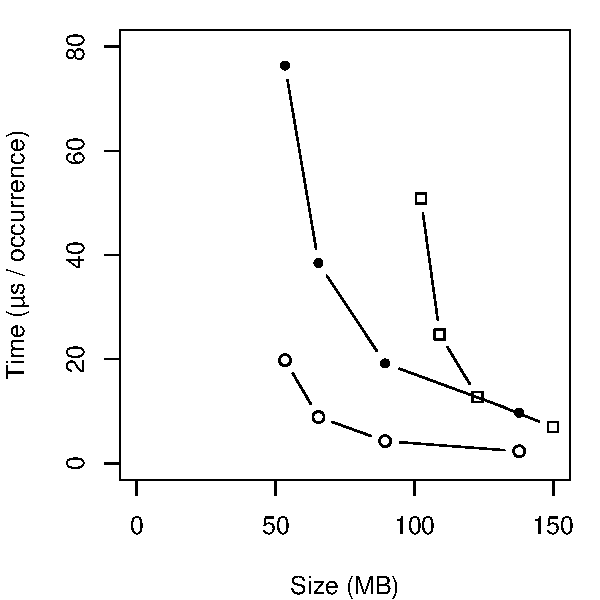
\includegraphics[width=.45\textwidth]{experiments/rlcsa/locate_para.pdf}
\hspace{5pt}
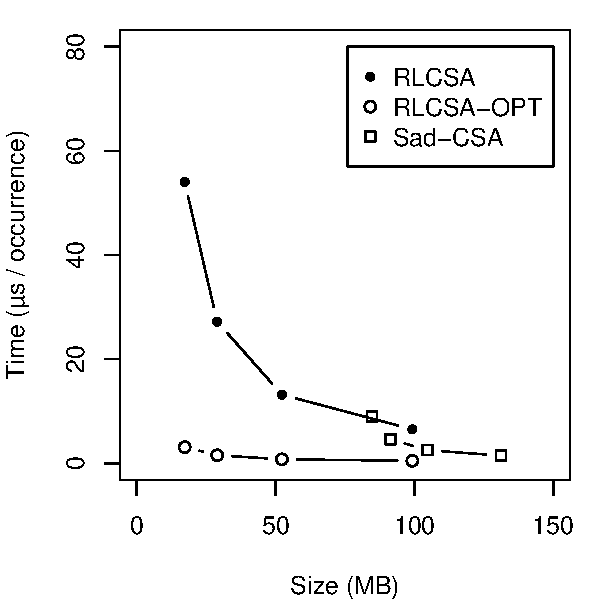
\includegraphics[width=.45\textwidth]{experiments/rlcsa/locate_fiwiki.pdf}
}

\caption{\emph{Locate} performance of RLCSA and \sadcsa\ on para (left) and fiwiki (right). Index sizes and average \locate\ times with sample rates $d = 32, 64, 128, 256$ on $50000$ patterns of length $20$.}\label{fig:rlcsa}
\end{figure}

The optimized \locate\ is $13$--$18$ times faster than the standard one on fiwiki, and about $4$ times faster on para. This shows that even though RLCSA is unable to compress the samples, unlike some other proposals \cite{Maekinen2010,Huang2010}, it can compensate this by using a small number of samples more efficiently, when the collection is highly repetitive.

In general, the optimizations depend on both the number and the length of the repetitions. Assume that we want to locate a pattern that occurs at the beginning of a repeated substring of length $l$, with $k$ copies in the collection. Then $k$ is an upper bound for the speedup from the optimizations, and the actual speedup depends on whether the significant prefixes of the sampled suffixes used in the \locate\ are within the repeated substring. If this is the case, then the suffixes remain lexicographically adjacent until the samples have been found. Otherwise the suffixes diverge at some point, limiting the speedup from locating all occurrences simultaneously.

It should be noted that \sadcsa\ has been optimized for \locate. The small blocks in the encoding of $\Psi$ contain a fixed number of values (\onebit{}s) each, and hence the correct block can be derived directly from the parameter value, avoiding one level of indirection. The sampling mechanism is also non-standard, storing one out of $d$ suffix array values instead of one out of $d$ text positions. This does not guarantee worst-case time bounds, but makes it much faster to determine whether the current suffix array value has been sampled.
\newpage


\section{Later indexes}

RLCSA was the first compressed index that was intended for indexing highly repetitive collections. Later papers on similar topics have used it as a reference point, against which the authors compare their results.

The self-index of Huang \etal{Huang2010} is based on a multiple alignment of similar sequences. The authors start with similar analysis as in Section~\ref{sect:runs}, and explicitly encode the differences between the sequences, while building a BWT-based index for the common segments in the sequences. When the number of differences is small, the index is smaller than RLCSA. The main reason for this is that the common segments are stored just once, while RLCSA uses $O(\log r)$ extra bits per run to encode the $r$ copies. Because of the complexity of the index, \find\ is slower than in regular BWT-based indexes. On the other hand, \locate\ can be much faster, if the pattern occurs mostly in the common segments.

The work of Claude \etal{Claude2009,Claude2010} develops self-indexes based on \emph{straight-line programs (SLP)} in general, and \emph{Re\nobreakdash-Pair} \cite{Larsson1999} in particular. Similar to \lzindex{}es, these indexes offer fast \locate, but do not support \find. A straight-line program is essentially a \emph{context-free grammar} in the \emph{Chomsky normal form} for a language containing a single sequence. In the grammar, each variable $X$ produces either two new variables $YZ$ or a character $c \in \Sigma$. One variant compresses the text with Re\nobreakdash-Pair, allowing fast random access to it, and uses a \emph{$q$\nobreakdash-gram index}, where the occurrence lists are differentially encoded and compressed with LZ77. Another variant uses the Re\nobreakdash-Pair encoding of the text directly as a self-index. Both variants offer better compression than RLCSA, if the text is very highly repetitive \cite{Claude2010}.

As already conjectured in the original paper describing RLCSA, a self-index based on LZ77 parsing offers better compression for highly repetitive sequences than RLCSA. The LZ77\nobreakdash-index of Kreft and Navarro \cite{Kreft2011} proves this conjecture. Like the other \lzindex{}es, the index is much larger than plain LZ77-compressed text. In practice, the LZ77\nobreakdash-index is smaller and offers faster \locate\ than RLCSA and SLP-based indexes on highly repetitive texts. The reason for better compression than SLP-based indexes is that while both approaches replace a repetition with a reference, SLPs have more overhead in encoding the original copy.

There have also been recent papers on compressing highly repetitive collections of sequences, while supporting the decompression of individual sequences or arbitrary substrings efficiently \cite{Kuruppu2010,Ferragina2010a,Kreft2010}. In these tasks, RLCSA is at disadvantage, as LZ77 compresses highly repetitive texts better than BWT, and the bit vector-based encoding of BWT also adds some overhead, when compared to direct compression. 



In order to convert the input data to the format required by BOSS (that is, in correct sorted order, including dummy edges and bit vectors), we use the following process.  We take care to ensure only subsets of data are needed in RAM at any one time during construction.

%First, 
%we read the header of the Cortex graph format, then iterate over the $(k-1)$-mers. For each $(k-1)$-mer, Cortex provides a bit matrix, where each row is a colour, and each
%column is a flag to indicate outgoing edges present in that colour. We invert this matrix to give us a bitmap representing the colours that each outgoing edge symbol is a member of.

Our construction algorithm takes as input the set of ($k$-mer, color-set) pairs present in the input sets of reads, or alternately, $k$-mer counts for each color which we convert to the former ourselves.
Here, color-set is a bit set indicating which samples the $k$-mer occurs in.
We provide the option to use the {\sc Cortex} frontend to generate the ($k$-mer, color-set). Unfortunately, this also limits the datasets to those that would run through {\sc Cortex}.  To overcome this, we provide the option to use a list of KMC2~\citep{KMC2} sorted $k$-mer counts as input.  With this option, the $k$-mers from each $k$-mer count file in native KMC2 binary format are streamed through a priority queue to produce the union of all $k$-mer sets; initially one $k$-mer from each file is tagged with  which file it originated from, and the ($k$-mer, file ID) pair is added to the queue.   The priority queue ensures the lexicographically smallest $k$-mer instances across all files can be popped off the queue consecutively.  All of the $k$-mer count files contributing a particular $k$-mer value have their corresponding color recorded as `1' bits in the bit set for that $k$-mer.  Both the $k$-mer and the bit set are then appended to vectors which optionally are allocated in external memory using the STXXL\footnote{\url{http://stxxl.sourceforge.net/}} library.   As each $k$-mer is popped off the queue, another $k$-mer is added to the queue to take the old $k$-mer's place (i.e. using the file identified by the popped $k$-mer's tag).  This process continues until all files are read in their entirety.  By both streaming data from the source files and streaming it to the external vectors, only a small amount of the data need exist in memory at a time; the priority queue will only contain the number of samples and only one row of the color matrix needs to exist in memory before being written out to disk.

%This effectively gives us ($k$-mer, color-set) pairs\footnote{In our current implementation, the color-set bitmaps were chosen to be 64 bits wide for simplicity, but can easily be extended to wider
%(or variable-length) bitmaps.}.

After constructing the initial union set of $k$-mers and their corresponding color rows, BOSS construction mostly continues as originally described by Bowe {\it et al.}.  The changes from the original construction algorithm are that most of the data optionally resides in external memory and the rows of the color matrix are permuted with their corresponding $k$-mers as they are sorted.  For each of the $k$-mers we generate the reverse complement (giving it the same color-set as its twin). Then, for each $k$-mer (including the reverse complements),
we sort the ($k$-mer, color-set) pairs by the first $k-1$ symbols (the source node of the edge) to give the $F$ table (from here, the colors are moved around with rows of $F$, but otherwise ignored until 
the final stage). Independently, we sort the $k$-mers (without the color-sets) by the last $k-1$ symbols (the destination node of the edge) to give the $L$ table.

With $F$ and $L$ tables computed, we calculate the set difference $F-L$ (comparing only the $(k-1)$-length prefixes and suffixes respectively), which tells us which nodes require incoming dummy edges. Each such node is then
shifted and prepended with $\$$ signs to create the required incoming dummy edges ($k-1$ each). These incoming dummy edges are then sorted by the first $k-1$ symbols.
Let this table of sorted dummy edges be $D$. Note that the set difference $L - F$ will give the nodes requiring outgoing dummy edges, but these do not require sorting, and so we can calculate it as is needed in the final stage.

Finally, we perform a three-way merge (by first $k-1$ symbols) $D$ with $F$, and $L-F$ (calculated on the fly). For each resulting edge, we keep track of runs of equal $k-1$ length prefixes,
and $k-2$ length suffixes of the source node, which allows us to calculate the $B_F$ and $B_L$ bit vectors, respectively. Next, we write the bit vectors, symbols from last column, and
count of the second to last column to a packed file on disk, and the colors to a separate file.   The color file is then either buffered in RAM and RRR encoded or optionally streamed from disk and then Elias-Fano encoded online (i.e. only the compressed version is ever resident).  The time bottleneck in the above process is clearly in sorting the $D$ and $F$ tables, which are of the same size, and are made up of elements of size $O(k)$. Thus, overall, construction of the data structure takes $O(k(|F|\log|F|))$ time.



%TODO: Asymptotics? We should also say that we use STXXL (which will give us EM sorting bounds)
% Reading: O(N) (# nodes) x O(sigma|C|)
% Sorting: O(|F| log |F|)
% F-L: O(|F|)
% Sort dummies: O(|D| log |D|)
% Final Merge: O(|F| + |D|) (|D| <= |F| -> O(|F|))


\chapter{Longest common prefix array}\label{chapter:lcp}

A \emph{compressed suffix tree (CST)} is a compressed data structure that provides similar functionality as the concrete suffix tree. While the exact list of operations varies from proposal to proposal, the extra functionality over a suffix array (see Definition~\ref{def:suffix array}) is mostly tree navigation and determining the length of the longest common prefix of the suffixes in a given subtree. The majority of compressed suffix tree proposals are actually compressed enhanced suffix arrays, combining a CSA, a compressed representation of the LCP array, and some representation of the suffix tree topology \cite{Sadakane2007,Fischer2009a,Maekinen2010,Ohlebusch2009,Ohlebusch2010}.

In this chapter, we investigate compressed LCP array representations and their space-efficient construction, based on Paper~III. We describe a LCP array sampling mechanism that can be used in a similar way as the suffix array samples in a compressed suffix array. For regular texts, this representation offers better time/space trade-offs than the earlier compressed representations. We also describe an algorithm for constructing the LCP array directly from a compressed suffix array.


\section{LCP array representations}\label{sect:lcp representations}

In a plain representation of the LCP array, each element is a $\log n$\nobreakdash-bit integer, for a total of $n \log n$ bits. Yet as the array can be derived from the text, it should be at least as compressible as the text itself. A number of different compressed representations have been proposed for the LCP array. Most of them are based on one or more of the three main ideas: variable-length codes, storing the array in text order, and sampling the array.

\paragraph{Variable-length codes.}

If the text is not highly repetitive, most of the LCP values are likely to be small. An easy way to utilize this to compress the LCP array  is to store small values (less than $255$) as $8$\nobreakdash-bit integers \cite{Abouelhoda2004}. Large values are marked with a $255$ in the array and stored explicitly as pairs $(i, \LCP[i])$. If a large value is needed, it can be found efficiently with binary searching. On typical texts, where large LCP values are rare, this representation takes approximately $8n$ bits of space.

A more advanced representation \cite{Canovas2010} is based on directly addressable codes \cite{Brisaboa2009}. The binary representation of each LCP value is broken into $b$\nobreakdash-bit chunks. The $i$th element of array $B_{1}$ contains the least significant chunk of $\LCP[i]$, followed by a bit indicating whether more chunks are needed to encode the value. Array $B_{2}$ contains the next chunks of LCP values larger than $2^{b}-1$, and a \rank\ index is built over the indicator bits of array $B_{1}$ to map the elements of $B_{1}$ to the corresponding elements of $B_{2}$. If more than $2b$ bits needed to encode the largest LCP values, arrays $B_{3}, B_{4}, \dotsc$ are built in a similar way. On typical texts, this representation takes $6n$ to $8n$ bits of space, with an average access time similar to one \rank\ or \select\ operation on a bit vector.

\paragraph{Permuted LCP array.}

While encoding each LCP value individually allows fast random access, the compression results are not that good. For better compression, we have to encode the values relative to other values. The key to this is the \emph{permuted LCP (PLCP) array} $\PLCP$ that stores the LCP values in text order. By using the PLCP array and the suffix array, we can retrieve any LCP value as $\LCP[i] = \PLCP[\SA[i]]$.

\begin{definition}\label{def:left match}
For text $T[1,n]$ and integer $i > 1$, the \emph{left match} of suffix $T[\SA[i],n]$ is the suffix $T[\SA[i-1],n]$.
\end{definition}

It follows that $\PLCP[j]$ is the length of the longest common prefix of suffix $T[j,n]$ and its left match $T[j',n]$. As $\lcp(T[j'+1,n], T[j+1,n])$ is a lower bound for $\PLCP[j+1]$ (unless $\PLCP[j] = 0$), we get the following lemma.

\begin{lemma}[\cite{Kasai2001,Kaerkkaeinen2009}]\label{lemma:plcp}
For $j \in \set{1, \dotsc, n-1}$, $\PLCP[j+1] \ge \PLCP[j] - 1$.
\end{lemma}

The definition and the lemma generalize for collections of texts as well.

An immediate consequence of Lemma~\ref{lemma:plcp} is that values $\PLCP[j] + 2j$ form a strictly increasing sequence. Hence the PLCP array can be encoded as bit vector $B_{L}$ of length $2n$. Individual PLCP values can then be retrieved as $\PLCP[j] = \select_{1}(B_{L}, j) - 2j$. In the original proposal of Sadakane \cite{Sadakane2007}, bit vector $B_{L}$ was  a succinct bit vector with constant-time \select, taking $2n + o(n)$ bits of space and allowing constant-time access to individual PLCP values.

For highly repetitive texts, a run-length encoded bit vector representation of the PLCP array provides even better compression.

\begin{definition}\label{def:minimal plcp values}
A PLCP value $\PLCP[j]$ is \emph{minimal}, if $j = n$ or $\PLCP[j] < \PLCP[j+1] + 1$. Value $\PLCP[j]$ is \emph{maximal}, if $j = 1$ or $\PLCP[j-1]$ is minimal.
\end{definition}

In a maximal run of \onebit{}s in bit vector $B_{L}$, the first \onebit{} encodes a maximal PLCP value, and the last \onebit{} encodes a minimal value.

\begin{lemma}\label{lemma:non-minimal plcp values}
Value $\PLCP[j]$ is non-minimal if and only if $\PLCP[j] = \PLCP[j+1] + 1$.
\end{lemma}

\begin{proof}
By definition, $j < n$ and $\PLCP[j] \ge \PLCP[j+1] + 1$ for non-minimal $\PLCP[j]$. By Lemma~\ref{lemma:plcp}, $\PLCP[j] \le \PLCP[j+1] + 1$.
\end{proof}

\begin{lemma}\label{lemma:plcp run heads}
The \onebit{} encoding $\PLCP[\SA[i]]$ in bit vector $B_{L}$ can be a run head only if $\BWT[i]$ is also a run head.
\end{lemma}

\begin{proof}
Assume that $\BWT[i-1] = \BWT[i]$, and let $\SA[i-1] = j'$ and $\SA[i] = j$. Suffix $T[j',n]$ is then the left match of suffix $T[j,n]$. As we have $LF(i-1) = LF(i) - 1$, we also have that $T[j'-1,n] = T[\SA[LF(i-1)],n]$ is the left match of suffix $T[j-1,n] = T[\SA[LF(i)], n]$. And as $T[j'-1] = \BWT[i-1] = \BWT[i] = T[j-1]$, it follows that $\PLCP[j-1] = \PLCP[j] + 1$. As $\PLCP[j-1]$ is non-minimal by Lemma~\ref{lemma:non-minimal plcp values}, $\PLCP[j]$ is non-maximal, and the \onebit{} encoding $\PLCP[j]$ is not a run head.
\end{proof}

\begin{corollary}[\cite{Fischer2009a}]\label{corollary:plcp runs}
The number of runs of \onebit{}s in bit vector $B_{L}$ is at most $R$.
\end{corollary}

For every run of \onebit{}s, there is exactly one minimal and one maximal PLCP value. Note that $\PLCP[\SA[i]]$ is not necessarily a maximal value, when $\BWT[i]$ is a run head. Experimental results suggest that the number of runs of \onebit{}s in bit vector $B_{L}$ is usually about $2R/3$ (see Section~\ref{sect:lcp experiments}).

Proposed run-length encoded representations of bit vector $B_{L}$ require at most $2R \log (n/R) + O(R) + o(n)$ \cite{Fischer2009a} or $2R \log (n/R) + O(R \log \log (n/R))$ \cite{Maekinen2010} bits of space, and provide fast access to individual PLCP values. The main drawback of all PLCP-based representations is that when used with a compressed suffix array, accessing \emph{LCP} values requires using \locate, which is an expensive operation.

\paragraph{Sampled PLCP representations.}

An alternative way to compress the PLCP array is to sample one out of $d'$ values and use the text and the suffix array to derive the rest \cite{Khmelev2004}. Assume that we have sampled $\PLCP[ad']$ and $\PLCP[(a+1)d']$, and we want to determine $\PLCP[ad' + b]$ for some $b < q$. Lemma~\ref{lemma:plcp} states that $\PLCP[ad'] - b \le \PLCP[ad' + b] \le \PLCP[(a+1)d'] + d' - b$, so at most $d' + \PLCP[(a+1)d'] - \PLCP[ad']$ character comparisons are required to determine the missing value. While the number of comparisons can be large in the worst case, the average number of character comparisons over the array is $O(d')$ \cite{Kaerkkaeinen2009}.

With a more careful selection of the sampled positions, we get similar trade-offs even in the worst case. In particular, we can store the samples in $o(n)$ bits, while requiring only $O(\log^{\delta} n)$ character comparisons in the worst case, for any $\delta > 0$ \cite{Fischer2009}. This solution is essentially the \select\ structure of bit vector $B_{L}$ without the bit vector itself.

While the sampled PLCP representations provide attractive trade-offs when used with a plain suffix array, they are slow with a compressed suffix array. In addition to requiring the expensive \locate\ operation to access LCP values, they also use the equally expensive \extract\ for character comparisons.


\section{Sampling the LCP array}

While increasing the number of suffix array samples increases the performance of PLCP-based representations, it also quickly eliminates the size advantage of those representations. A sampled LCP representation can offer better time/space trade-offs, as individual LCP samples tend to be smaller than suffix array samples.

Assume that we have sampled the at most $R$ \emph{minimal} PLCP values, where $\PLCP[j] < \PLCP[j+1] + 1$. If we store these samples in suffix array order in the same way as suffix array samples, we can use a similar mechanism to retrieve the rest of the values. If $\LCP[i]$ has not been sampled, we proceed to position $\Psi(i)$ and check if $\LCP[\Psi(i)]$ has been sampled. If $\LCP[\Psi^{k}(i)]$ is the first sampled position we encounter, then $\LCP[i] = \LCP[\Psi^{k}(i)] + k$. This follows from the fact that $\LCP[\Psi^{k'}(i)]$ is a non-minimal PLCP value for all $k' < k$, and hence $\LCP[\Psi^{k'}(i)] = \PLCP[\SA[i] + k'] = \PLCP[\SA[i] + k' + 1] + 1 = \LCP[\Psi^{k'+1}(i)] + 1$ by Lemma~\ref{lemma:non-minimal plcp values}.

\begin{lemma}[\cite{Kaerkkaeinen2009}]\label{lemma:minimal plcp values}
For a text of length $n$, the sum of minimal or maximal PLCP values is at most $2n \log n$.
\end{lemma}

The worst case occurs in random texts, where most of the PLCP values are both maximal and minimal, and the average value is $\Theta(\log_{\sigma} n)$ (see the analysis in Section~\ref{sect:runs}). For a binary de Bruijn sequence, the sum of maximal values (with a looser definition, where Lemma~\ref{lemma:plcp run heads} holds in both directions) is $(n/2) \log n - O(n)$ \cite{Kaerkkaeinen2009}, making the bound asymptotically tight. In highly repetitive texts, the sum of minimal values tends to be less than $n$ (see Section~\ref{sect:lcp experiments}).

If we use the bit vector of Gupta \etal{Gupta2007} to mark the sampled positions, the vector takes $(1 + O(1 / \log R)) R \log (n/R) + O(R \log \log (n / R))$ bits of space in the worst case. As the sum of the samples is at most $2n \log n$, we can concatenate the binary representations of the samples in at most $R \log (2n \log n / R) + R$ bits. The two-level storage scheme of Ferragina and Venturini \cite{Ferragina2007} allows constant-time access to the samples by using $O(R \log \log n / \log n)$ bits of extra space. Overall, the samples require
$$
\left( 2 + O\left( \frac{1}{\log R} \right) \right) R \log \frac{n}{R} +
O\left( R \log \log \frac{n}{R} \right)
$$
bits of space, which is almost the same as for one of the run-length encoded PLCP proposals \cite{Maekinen2010}.

To guarantee worst-case behavior and to improve the performance with highly repetitive texts, where $R \ll n$, we also sample one out of $d' > 0$ PLCP values, when the successive minimal values are spaced more than $d'$ positions apart. With the pessimistic assumption that each of these extra samples is large, requiring $\log n$ bits, the size bound becomes
$$
\left( 1 + O\left( \frac{1}{\log n_{S}} \right) \right) n_{S} \log \frac{n}{n_{S}} +
R \log \frac{n}{R} +
\frac{n \log n}{d'} +
O\left( n_{S} \log \log \frac{n}{n_{S}} \right)
$$
bits, where $n_{S} \le R + n/d'$ is the number of samples. In practice, an extra sample $\PLCP[j]$ requires roughly $\log \PLCP[j]$ bits and a mark in the bit vector, while an extra suffix array sample requires $2 \log (n/d)$ bits in addition to the mark, where $d$ is the suffix array sample rate. Hence with typical sample rates, adding extra LCP samples is cheaper than adding the same number of suffix array samples.

\begin{theorem}\label{theorem:sampled lcp}
Let $T[1,n]$ be a text, and let $d' > 0$ be an integer. The LCP samples for text $T$ with sample rate $d'$ require
$$
O\left(  n_{S} \log \frac{n}{n_{S}} \right) + \frac{n \log n}{d'}
$$
bits of space, where $n_{S} \le R + n/d'$ is the number of samples, and $R$ is the number of equal letter runs in the Burrows-Wheeler transform of text $T$. A compressed suffix array that computes $\Psi$ in $t_{\Psi}$ time can use the samples to access any element of the LCP array in $O(d' \cdot (t_{\Psi} + o(\log n)))$ time.
\end{theorem}


\section{Space-efficient LCP array construction}

Kasai \etal{Kasai2001} introduced the first linear-time LCP array construction algorithm. As the algorithm requires the suffix array in memory, it uses $\Theta(n \log n)$ bits of space for a text of length $n$. Yet as the LCP array can be compressed into $2n + o(n)$ bits or even less, this greatly restricts the size of the texts with which the LCP array can be used. Later developments concentrated on reducing the working space to $O(n \log \sigma)$ bits \cite{Puglisi2008,Kaerkkaeinen2009,Gog2011,Beller2011} or making the construction faster in practice \cite{Kaerkkaeinen2009,Gog2011,Fischer2011}.

The fastest algorithm so far is the one by Fischer \cite{Fischer2011}. Based on a suffix array construction algorithm using induced sorting \cite{Nong2009a}, the algorithm works in linear time, yet requires $\Theta(n \log n)$ bits of working space. Another interesting algorithm is the one by Beller \etal{Beller2011} that builds the LCP array directly from a compressed suffix array. On a conceptual level, the algorithm is based on repeating the following for $k = 0, 1, \dotsc$.

\begin{enumerate}

\item For all patterns $P$ of length $k$, let $[sp_{P}, ep_{P}]$ be the suffix array range containing the occurrences of the pattern. Assume that set $Q_{k}$ contains all these ranges.

\item Use backward searching to determine set $Q_{k+1}$ from set $Q_{k}$.

\item For each range $[sp, ep] \in Q_{k+1}$, set $\LCP[ep+1] \leftarrow k$, unless $\LCP[ep+1]$ has already been defined.

\end{enumerate}

A practical variant of the algorithm works in $O(n \log n)$ time and uses roughly $n$ bytes of working space in addition to the compressed suffix array. The LCP array is written directly to disk in several passes. While the algorithm is reasonably fast and space-efficient, it cannot be used for constructing the LCP array for texts that are too large to fit into memory. This is in contrast to the compressed suffix arrays, for which such algorithms exist (see Chapter~\ref{chapter:construction}).

By starting from the \emph{irreducible LCP algorithm} of Kärkkäinen \etal{Kaerkkaeinen2009}, we can design an LCP array construction algorithm that uses negligible working space in addition to the compressed suffix array and the compressed (P)LCP representation. The irreducible LCP algorithm finds the irreducible (maximal) PLCP values, computes them directly, and uses Lemma~\ref{lemma:non-minimal plcp values} to derive the rest of the values. As the sum of maximal PLCP values is at most $2n \log n$, the algorithm works in $O(n \log n)$ time. The PLCP values are computed in text order, making it possible to build any compressed PLCP representation directly.

The original irreducible LCP algorithm uses the text and the suffix array to identify the maximal values. With a compressed suffix array, we want to identify the irreducible values using function $\Psi$ in one pass over the text. Additionally, as computing the irreducible values also involves scanning the text forward using $\Psi$, we can avoid redundant work by finding minimal instead of maximal PLCP values.

From Lemma~\ref{lemma:plcp run heads}, we can derive the following result by noting that $\PLCP[j]$ is minimal if $\PLCP[j+1]$ is maximal.

\begin{lemma}\label{lemma:identifying minimal plcp values}
Let $\SA[i] = j$. Value $\PLCP[j]$ can be minimal only if $j = n$ or if $\BWT[\Psi(i)]$ is a run head.
\end{lemma}

Let $c$ be a character such that $C[c] < i \le C[c+1]$. As we compute $\Psi(i) = \mselect_{c}(\BWT, i - C[c])$, we know that $\BWT[\Psi(i)]$ is a run head if we use a run head in $\BWT$ (or in bit vector $B_{c}$) to compute $\Psi(i)$. Equivalently, $\BWT[\Psi(i)]$ is a run head if and only if $\mchar(i-1) \ne \mchar(i)$ or $\Psi(i-1) \ne \Psi(i) - 1$.

While Lemma~\ref{lemma:identifying minimal plcp values} produces false positives, we can identify true minimal values by buffering the previous candidate, until we find the next possibly minimal value. The modified irreducible LCP algorithm can be seen in Figure~\ref{fig:irreducible lcp algorithm}.

\begin{figure}
\begin{tabbing}
mm\=mm\=mm\=mm\= \kill
\> \textbf{function} $\lcp(i)$ \\
\> \> $(i', k) \leftarrow (i-1, 0)$ \\
\> \> $c \leftarrow \mchar(i)$ \\
\> \> \textbf{while} $i' \in C_{c}$ \\
\> \> \> $(i', i, k) \leftarrow (\Psi(i'), \Psi(i), k + 1)$ \\
\> \> \> $c \leftarrow \mchar(i)$ \\
\> \> \textbf{return} $k$ \\
\\
\> \textbf{function} $\operatorname{irreducibleLCP}(\SA^{-1}[1])$ \\
\> \> $\PLCP[1] \leftarrow 0$ \\
\> \> $(i, j, j') \leftarrow (\SA^{-1}[1], 1, 2)$ \\
\> \> \textbf{while} $j < n$ \\
\> \> \> $c \leftarrow \mchar(i)$ \\
\> \> \> \textbf{if} $i-1 \not\in C_{c}$ \textbf{or} $\Psi(i-1) \ne \Psi(i) - 1$ \\
\> \> \> \> $x \leftarrow \lcp(\Psi(i))$ \\
\> \> \> \> $\PLCP[j', j+1] \leftarrow (x + j+1 - j', \dotsc, x)$ \\
\> \> \> \> $j' \leftarrow j + 2$ \\
\> \> \> $(i, j) \leftarrow (\Psi(i), j + 1)$ \\
\> \> \textbf{return} $\PLCP$ 
\end{tabbing}

\caption{The irreducible LCP algorithm for computing the PLCP array directly from a compressed suffix array. The algorithm maintains an invariant that $\SA[i] = j$, while $\PLCP[j']$ is the maximal value in the current run.}\label{fig:irreducible lcp algorithm}
\end{figure}

A two-pass variant of the same algorithm can be used to sample the LCP array. In the first pass, we scan the CSA in suffix array order, and find the minimal samples. As the samples are output in suffix array order, we can compress them immediately, using negligible working space. The second pass is in text order, as in the original algorithm. We output one out of $d'$ consecutive non-minimal values as pairs $(i, \LCP[i])$, deriving $\LCP[i]$ from the next sample. Once the non-minimal samples have been determined, we sort them in suffix array order, and merge them with the minimal samples.

\begin{theorem}\label{theorem:irreducible lcp algorithm}
Given a compressed suffix array for a text of length $n$, the irreducible LCP algorithm computes the PLCP array in negligible working space in addition to the CSA and the PLCP array. The running time of the algorithm is equivalent to extracting $O(n \log n)$ characters from the text using the CSA. A two-pass version of the algorithm samples the LCP array with sample rate $d' > 0$ in the same time bound, while using $O((n/d') \log n)$ bits of additional working space.
\end{theorem}
\newpage


\section{Implementation and experiments}\label{sect:lcp experiments}

LCP samples, bit vector encodings of the PLCP array, and their construction algorithms have been implemented as a part of RLCSA (see Chapter~\ref{chapter:rlcsa}). For PLCP, we use a run-length encoded bit vector with highly repetitive data sets, and a succinct bit vector with regular data sets. For marking the sampled LCP positions, we similarly use a gap encoded bit vector with highly repetitive data sets, and a succinct vector with the regular ones. The sampled values are encoded with \deltacode{}s, and stored in a stripped-down version of the gap encoded bit vector for fast access.

The succinct bit vector is a practical implementation designed for current hardware. For \rank, we divide the vector into $256$\nobreakdash-bit blocks, and store the number of \onebit{}s before each block in $\log n$ bits. Solving \rank{} then requires retrieving the stored value for the correct block, and counting the number of $1$-bits in the block up to the queried position using the $64$-bit $\popcount$ function provided in GCC. The function compiles either into a single instruction or a small subroutine, depending on architecture.

For \select, the implementation uses two levels of indexes. The first one stores $n/256$ pointers to blocks that contain the \onebit{} of rank $i \cdot 256n_{1}/n + 1$, for $i = 0$ to $n/256 - 1$. With this index, we get a range of blocks that contains the queried \onebit. If the range spans more than $16$ blocks, we use binary search in the \rank{} index to narrow it down. When the range becomes short enough, we continue with linear search in the \rank{} index to find the correct block, and resort to $\popcount$ to compute the answer within the block.

To avoid redundant work in LCP sampling and PLCP construction, we interleave the computation of minimal values with the main loop. When sampling the LCP array, we make both of the passes in text order, and store all samples in an array of pairs $(i, \LCP[i])$ before compressing them.

For the experiments, we used the same system as in Section~\ref{sect:rlcsa experiments}. Only once core was used in the experiments. We used the same four data sets as in Paper~III. As regular data sets, we used human DNA sequences (dna) and English language texts (english) from the Pizza \& Chili Corpus \cite{Ferragina2009a}. As highly repetitive data sets, we used Finnish language Wikipedia with full version history (fiwiki) and the genomes of 36 strains of \emph{Saccharomyces paradoxus} (para) (see also Chapter~\ref{chapter:rlcsa}). When the data set was much larger than 400 megabytes, a 400 MB prefix was used instead. Further information on the data sets can be found in Table~\ref{table:lcp data sets}.

\begin{table}
\centering
\renewcommand{\tabcolsep}{.1cm}
\begin{tabular}{lccccccccc}
\hline\noalign{\smallskip}
 & & & & \multicolumn{2}{c}{\textbf{Minimal}} & & \multicolumn{3}{c}{\textbf{Construction}} \\
\textbf{Data set} & \textbf{Size} & \textbf{Runs} & & \textbf{Number} & \textbf{Sum} & & \textbf{PLCP} & \textbf{Samples} & \textbf{Induced} \\
\noalign{\smallskip}
\hline
\noalign{\smallskip}
dna     & 385 & 243.49 & & 158.55 & 2215 & & 2402 & 2695 & 47 \\
english & 400 & 156.35 & &  99.26 & 1052 & & 1181 & 1471 & 76 \\
fiwiki  & 400 &   1.79 & &   1.15 &  117 & &  210 &  365 & 46 \\
para    & 409 &  15.64 & &  10.05 &  299 & &  374 &  590 & 55 \\
\noalign{\smallskip}
\hline
\end{tabular}

\caption{Data sets used in LCP experiments. Size in megabytes, millions of runs in BWT, number and sum of minimal samples in millions, and construction time in seconds. Construction times for PLCP and (LCP) Samples are from using the irreducible LCP algorithm, while Induced is for building the LCP array with the algorithm of Fischer \cite{Fischer2011}, which is currently the fastest LCP construction algorithm.}\label{table:lcp data sets}
\end{table}

The construction times reported in Table~\ref{table:lcp data sets} are for the highest number of SA and LCP samples. Note that sample rates had no significant impact on construction times. With the regular data sets, the irreducible LCP algorithm was very slow, as its time complexity scales with the sum of minimal PLCP values. A parallel version that scans different sequences in different threads might still be as fast as direct CSA construction (see Chapter~\ref{chapter:construction}), as the basic CSA operations parallelize well. The algorithm was much faster with the highly repetitive data sets, while still being $5$ to $10$ times slower than the LCP construction algorithm of Fischer \cite{Fischer2011}.

As noted in Section~\ref{sect:lcp representations}, the number of minimal PLCP values was roughly $2/3$ times the number of equal letter runs in the Burrows-Wheeler transform of the text. As the number of minimal PCLP values is the same as the number of runs of \onebit{}s in the PLCP vector $B_{L}$, this means that the size bounds for the run-length encoded PLCP variants are significantly larger than the size in practice.

To compare the time/space trade-offs offered by PLCP bit vectors and LCP samples, we built RLCSA with sample rates $d = 8, 16, 32, 64$ for the regular data sets, and $d = 32, 64, 128, 256$ for the highly repetitive data sets. We used LCP sample rates $d' = 8, 16$ for the regular data sets, and $d' = 16, 32, 64$ for the highly repetitive ones. Instead of measuring the average time required for a random LCP query, we used a measure that is independent of the underlying CSA implementation, counting the average number of steps of $\Psi$ required to find a sampled SA or LCP position. The results can be seen in Figure~\ref{fig:lcp results}. As a lower bound for the size of any PLCP-based representation, we also included the results for \locate{} in the figures.

\begin{figure}
\centerline{
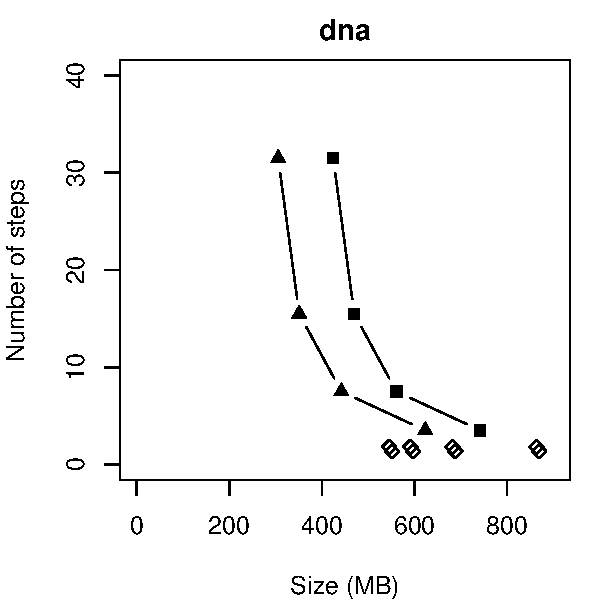
\includegraphics[width=.45\textwidth]{experiments/lcp/dna.pdf}
\hspace{5pt}
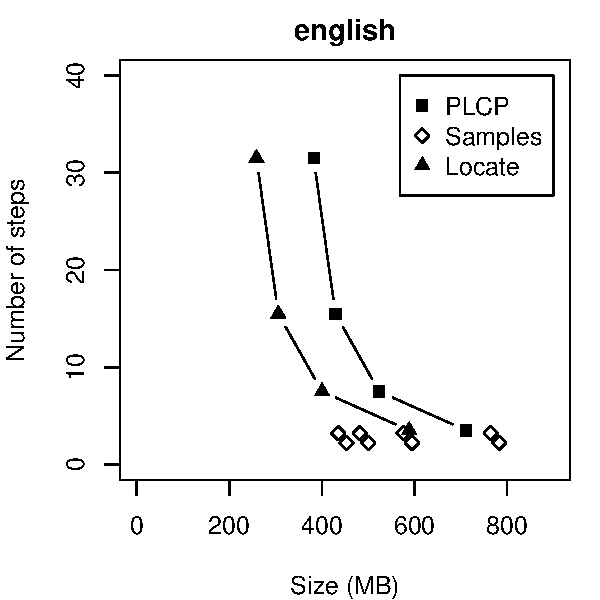
\includegraphics[width=.45\textwidth]{experiments/lcp/english.pdf}}

\centerline{
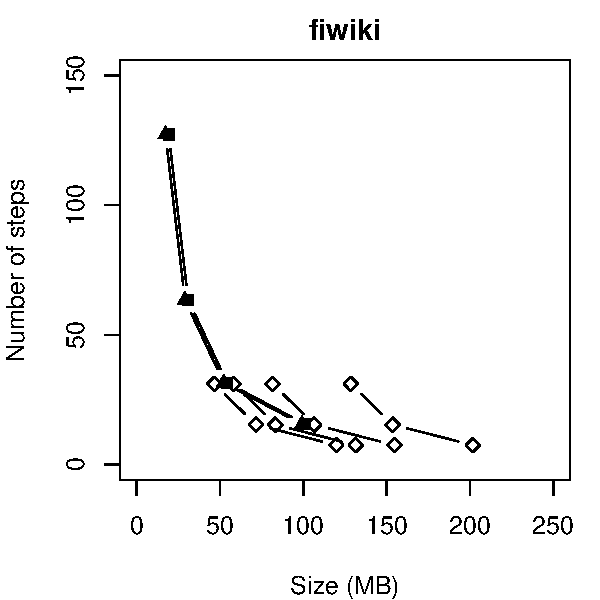
\includegraphics[width=.45\textwidth]{experiments/lcp/fiwiki.pdf}
\hspace{5pt}
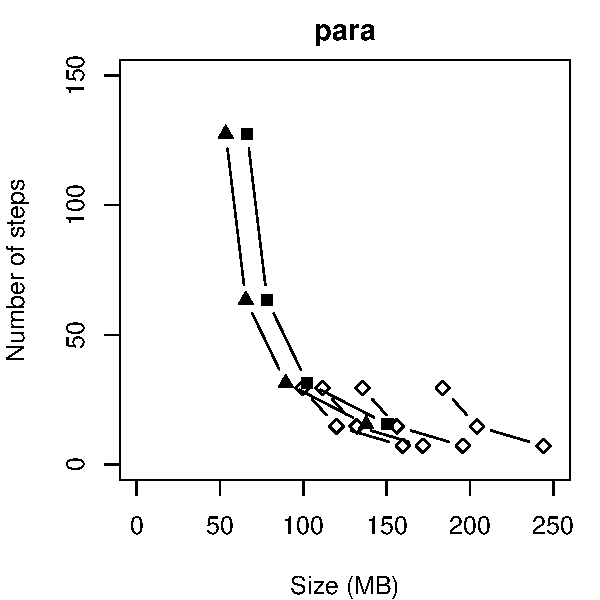
\includegraphics[width=.45\textwidth]{experiments/lcp/para.pdf}
}
\caption{Experimental results for $10^{6}$ random LCP queries with LCP samples and PLCP, with $10^{6}$ random \locate{} queries as a lower bound for any PLCP-based representation. Index size in megabytes and the average number of steps required to reach a SA/LCP sample. The results with LCP samples have been grouped by SA sample rate.}
\label{fig:lcp results}
\end{figure}

With the regular data sets and sparse SA sampling, the performance of LCP samples was superior to the PLCP-based approach, while increasing the overall index size only slightly. As $25\%$ (english) to $40\%$ (dna) of text positions were sampled, a sampled position was found in a couple of steps most of the time. With denser suffix array sampling, this advantage mostly disappeared, as the \locate{} queries were no longer that expensive.

As there were only a few minimal samples in the highly repetitive data sets (see Table~\ref{table:lcp data sets}), the solution using LCP samples relied mostly on the non-minimal extra samples. This made the LCP samples significantly larger than the run-length encoded PLCP bit vector. While the LCP samples still offered better time/space trade-offs than any PLCP-based approach in some cases, the improvement was not significantly better than what could be achieved by denser suffix array sampling.

We also measured the average number of steps required for computing the LCP values directly. As there were long repetitions even in the regular data sets, the results (2424 steps in dna and 5786 steps in english) were not competitive with the other approaches. Still, as many of the minimal samples are small, it should be possible to decrease the size of the samples without sacrificing too much performance by storing only large minimal samples, and computing the small ones directly when required.


\chapter{Generalized compressed suffix array}\label{chapter:gcsa}

The compressed suffix arrays discussed so far index either single sequences or collections of sequences. This is not a fundamental limitation, however. In this chapter, based on Paper~IV, we generalize the compressed suffix arrays to handle a certain class finite automata. This class of automata can recognize all finite languages and some infinite languages as well.

Backward searching using BWT is based on the following property: text positions containing character $c$ are sorted in the same order as text positions preceded by character $c$. If we consider the sequence a finite automaton, we could say that nodes labeled with character $c$ are sorted in the same order as those nodes with a predecessor labeled with character $c$. To use this idea to index finite automata, we need to solve two problems: handling nodes with multiple predecessors or successors (Section~\ref{sect:gcsa}), and constructing an automaton that can be sorted in the desired way (Section~\ref{sect:gcsa construction}).

In the general case, the sorted automaton can be exponentially larger than the minimal deterministic automaton recognizing the same language. However, if only a small fraction of the nodes of the minimal automaton have multiple successors, most of the nodes can be sorted by the label of the unique path of length $k$ (for some $k > 0$) starting from the node. For these languages, the sorted automaton is not much larger than the minimal one. An important example of this kind of automata are those arising from a reference sequence and a set of substitutions, insertions, and deletions, or from a multiple alignment of sequences. In the latter case, the automaton will recognize not only the original sequences, but all their plausible recombinations as well.
\newpage


\section{Indexing finite languages}\label{sect:gcsa}

The {\em XBW transform} \cite{Ferragina2009b} is a generalization of the Burrows-Wheeler transform for labeled trees, where leaf nodes and internal nodes are labeled with different alphabets. Each internal node of the tree is represented as a concatenation of the labels of its children. These representations, sorted in lexicographic order according to the path labels from the node to the root, form sequence $\BWT$. The starting position of each internal node in $\BWT$ is marked by an \onebit{} in bit vector $F$, so that the node with lexicographic rank $i$ can be found as $\BWT[\mselect_{1}(F,i), \mselect_{1}(F,i+1) - 1]$.

XBW supports tree navigation with generalizations of functions $LF$ and $\Psi$. In downward functions such as $LF$, the lexicographic ranks returned by the regular versions of the functions are converted into BWT ranges by using \select{} on bit vector $F$, as above. Upward functions such as $\Psi$ work in the opposite way, converting BWT ranges into lexicographic ranks by using \rank{} on bit vector $F$, before calling the regular version of the function.

\paragraph{Generalization for finite automata.}

Bit vector $F$, mapping lexicographic ranks into BWT ranges, allows a single node to have multiple predecessors. We can use a similar idea to allow multiple successors, extending XBW from trees to finite automata. The idea is to use another bit vector $M$ to encode the number of outgoing edges, so that the node with lexicographic rank $i$ has $\mselect_{1}(M,i+1) - \mselect_{1}(M,i)$ outgoing edges.\footnote{This definition of bit vector $M$ makes the generalization simpler than the original definition.} For convenience, we assume that the final node $V_{\abs{V}}$ has a single outgoing edge to the initial node $V_{1}$.

Backward navigation ($LF$) first uses bit vector $F$ to convert lexicographic ranks into a BWT range, then calls the regular version of the function, and finally uses bit vector $M$ to convert the edge range into lexicographic ranks. Forward navigation ($\Psi$) uses bit vectors $M$ and $F$ in the opposite way. See Figure~\ref{fig:gcsa navigation} for pseudocode for basic navigation functions, and below for exact definitions of the functions.

\begin{figure}[t!]\centering
\begin{tabbing}
mm\=mm\=mm\= \kill
{\bf function} $\operatorname{LF}([sp,ep], c)$ \\
\> $[sp, ep] \leftarrow [\mselect_{1}(F,sp), \mselect_{1}(F,ep+1) - 1]$ \\
\> $[sp, ep] \leftarrow [C[c] + \mrank_{c}(\BWT, sp - 1) + 1, C[c] + \mrank_{c}(\BWT, ep)]$ \\
\> $[sp, ep] \leftarrow [\mrank_{1}(M,sp), \mrank_{1}(M,ep)]$ \\
\> {\bf return} $[sp,ep]$ \\
\\
{\bf function} $\Psi(i, j)$ \\
\> $c \leftarrow \mchar(i)$ \\
\> $i \leftarrow \mselect_{1}(M,i) + j - 1$ \\
\> $i \leftarrow \mselect_{c}(\BWT, i - C[c])$ \\
\> $i \leftarrow \mrank_{1}(F,i)$ \\
\> {\bf return} $i$
\end{tabbing}

\caption{Pseudocode for the basic navigation functions $LF$ and $\Psi$.}\label{fig:gcsa navigation}
\end{figure}

\paragraph{Definitions.}

As mentioned in the beginning of the chapter, the automaton must have a certain property in order for functions $LF$ and $\Psi$ to work. We call this property prefix-range-sortedness.

\begin{definition}\label{def:prefix-range-sorted}
Let $A = (V, E)$ be a finite automaton, and let $v \in V$ be a node. Let $rng(v)$ be the smallest (open, semiopen, or closed) lexicographic range containing all suffixes that can be recognized from node $v$. Node $v$ is {\em prefix-range-sorted}, if no suffix $S \in rng(v)$ is recognized from any other node $v' \ne v$. Automaton $A$ is prefix-range-sorted, if all nodes are prefix-range-sorted.
\end{definition}

In the following, we use a stronger definition to simplify the discussion. The results for prefix-sorted automata generalize for prefix-range-sorted automata as well.

\begin{definition}\label{def:prefix-sorted}
Let $A$ be a finite automaton, and let $v \in V$ be a node. Node $v$ is {\em prefix-sorted} by prefix $p(v)$, if the labels of all paths from $v$ to $v_{\abs{V}}$ share a common prefix $p(v)$, and no path from any other node $u \ne v$ to $v_{\abs{V}}$ has $p(v)$ as a prefix of its label. Automaton $A$ is prefix-sorted, if all nodes are prefix-sorted.
\end{definition}

We can use the prefixes $p(v)$ to sort the nodes of a prefix-sorted automaton in lexicographic order. If we do so, then we have also sorted the outgoing edges $(u,v)$ using sequences $\ell(u) p(v)$ as sort keys, and the edge encoded by bit $M[i]$ has lexicographic rank $i$. This is the key for functions $LF$ and $\Psi$ to work properly. For any given character $c$, all outgoing edges from nodes with label $c$ are lexicographically adjacent, and they are sorted by prefix $p(v)$ of the destination node. Similarly, all occurrences of character $c$ in $\BWT$ encode an incoming edge from a node with label $c$, and these edges are also sorted by prefix $p(v)$ of the destination node. Hence the incoming edge labeled by the $j$th occurrence of character $c$ is the same edge as the outgoing edge of rank $C[c] + j$, and the other way around. Note that $C[c]$ stores the number of occurrences of characters smaller than $c$ in $\BWT$, not the number of nodes with label smaller than $c$.

\paragraph{Operations.}

We define the basic navigation functions in the following way.
\begin{itemize}
\item $LF([sp,ep], c)$ is the lexicographic range of nodes with label $c$ that have a successor in the lexicographic range $[sp,ep]$. This is essentially a step of backward searching with character $c$.
\item $\Psi(i, j)$ is the lexicographic rank of the $j$th successor of the node with lexicographic rank $i$.
\item $\mchar(i)$ is the label of the node with lexicographic rank $i$.
\end{itemize}

These operations can be used to support the following generalization of suffix array functionality (see Definition~\ref{def:suffix array}).
\begin{itemize}
\item \find($P$) returns the lexicographic range $[sp, ep]$ of nodes recognizing any suffix that has pattern $P$ as its prefix.
\item \locate($i$) returns a numerical value corresponding to the node with lexicographic rank $i$.
\item \extract($i, \Path$) returns the label of path $\Path$ starting from the node with lexicographic rank $i$.
\end{itemize}

We can support \find{} by replacing the first two lines of the loop body in Figure~\ref{fig:backward searching} with function $LF$ from Figure~\ref{fig:gcsa navigation}.

For \locate, we assume that there is a (not necessarily unique) numerical value $id(v)$ attached to each node $v \in V$. Examples of these values include node ids (so that $id(v_{i}) = i$) and positions in a multiple alignment. To avoid excessive sampling of node values, $id(v)$ should be $id(u) + 1$ whenever $(u,v)$ is the only outgoing edge from $u$ and the only incoming edge to $v$.

We sample $id(u)$, if there are multiple outgoing edges from node $u$, or if $id(v) \ne id(u) + 1$ for the only outgoing edge $(u, v)$. We also sample one out of $d$ node values, given sample rate $d > 0$, on paths of at least $d$ nodes without any samples. The sampled values are stored in the same order as the nodes, and their positions are marked in bit vector $B_{s}$.

As we have sampled all nodes with multiple successors, we can use the \locate{} algorithm of the CSA family directly with our new function $\Psi$. To retrieve $id(u)$ for node $u$ of lexicographic rank $i$, we first check if $B_{s}[i] = 1$, and return sample $rank_{1}(B_{s}, i)$, if this is the case. Otherwise we follow the only outgoing edge $(u,v)$ by using function $\Psi$, and continue from node $v$. When we find a sampled node $w$, we return $id(w) - k$, where $k$ is the number of steps taken by using $\Psi$.

In \extract, we assume that the description of path $\Path$ allows us to determine in constant time, which outgoing edge we should take, and have we already finished the path. With such description, we can use function $\Psi$ to move forward on the path, and function $\mchar(\cdot)$ to read the next character of the path label. The algorithm is similar to the \extract{} algorithm of the CSA family, with the exception that we already know the lexicographic rank of the initial node. This is because we might be using a node value scheme that does not allow mapping node values to lexicographic ranks.

We call a compressed self-index based on this generalization of the XBW transform a \emph{generalized compressed suffix array (GCSA)}. As each step of $LF$ and $\Psi$ requires both \rank{} and \select, we get the following generalization of Theorem~\ref{theorem:csa}.

\begin{theorem}\label{theorem:gcsa}
Let \rank\ and \select\ on binary sequences take $t_{R}$ and $t_{S}$ time, respectively. Then a generalized compressed suffix array with sample rate $d$ supports \find$(P)$ in $O(\abs{P} \cdot (t_{R} + t_{S}))$ time, \locate\ in $O(d \cdot (t_{R} + t_{S}))$ time, and \extract$(i, \Path)$ in $O(\abs{\Path}(t_{R} + t_{S}))$ time.
\end{theorem}

\paragraph{A better encoding.}

Recall that the size bound of RLCSA (Theorem~\ref{theorem:rlcsa}) is worse than for plain run-length encoding of the BWT (Section~\ref{sect:compression}). This is because RLCSA has to encode each character of $\BWT$ with either a \zerobit{} or an \onebit{} in every bit vector $B_{c}$, while the run-length encoding encodes each character only once. In GCSA, we can use this redundancy for our advantage.

As a prefix-range sorted automaton is reverse deterministic, each node can have at most one predecessor with a certain label. Hence the section of $\BWT$ corresponding to a node can have at most one occurrence of each character, meaning that we can put all these predecessor labels into the same position in bit vectors $B_{c}$. As the bit $B_{c}[i]$ now determines, whether the node with lexicographic rank $i$ has a predecessor with label $c$, we no longer have to use bit vector $F$ to map between lexicographic ranks and BWT ranges. This is a major speedup in practice, as we get rid of one third of bit vector operations.


\section{Construction algorithm}\label{sect:gcsa construction}

A straightforward way of constructing a prefix-sorted automaton from a finite automaton recognizing a finite language is via a prefix-doubling algorithm (see Section~\ref{sect:construction implementation}). The algorithm consists mostly of sorting, scanning, and database joins. Hence it can be efficiently implemented in parallel, distributed, and external memory settings.

\begin{theorem}
Assume we have a length $n$ multiple alignment of $r$ sequences over alphabet of size $\sigma$. We can build a prefix-range-sorted automaton recognizing all paths through the alignment in $O(nr + \abs{V'} \log n + \abs{E'})$ time and $O(nr \log \sigma + \abs{V'} \log \abs{V'} + \abs{E'} \log \abs{E'})$ bits of space, where $V'$ and $E'$ are the largest intermediate sets of nodes and edges, respectively.
\end{theorem}

\begin{proof}
From Lemmas \ref{lemma:automaton construction}, \ref{lemma:node construction}, and \ref{lemma:edge construction} below.
\end{proof}

The sizes of the largest intermediate sets of nodes and edges are analyzed in a restricted model in Section~\ref{sect:gcsa analysis}. An example of construction can be seen in Figures~\ref{fig:automaton} and \ref{fig:prefix-sorted automaton} and Table~\ref{table:gcsa example}.

\begin{figure}
\centerline{\includegraphics{figures/automaton.pdf}}
\caption{A reverse deterministic automaton corresponding to the first 10 positions of the multiple alignment in Figure~\ref{fig:multiple alignment}.} 
\label{fig:automaton}
\end{figure}

\begin{figure}
\centerline{\includegraphics{figures/sorted.pdf}}
\caption{A prefix-sorted automaton built for the automaton in Figure~\ref{fig:automaton}. The strings above nodes are prefixes $p(v)$.} 
\label{fig:prefix-sorted automaton}
\end{figure}

\begin{table}
\centering
\renewcommand{\tabcolsep}{.05cm}
\texttt{
\begin{tabular}{cccccccccccccccccccc}
\hline\noalign{\smallskip}
       & & \$  & ACC & ACG & ACTA & ACTG & AG & AT & CC & CG & CTA & CTG & G\$ & GA   & GT & TA  & TG\$ & TGT & \# \\
\noalign{\smallskip}
\hline
\noalign{\smallskip}
$\BWT$ & & G & T & G & G & T & T & G & A  & A  & A & AC & AT & \#  & CT & CG  & C & A & \$ \\
$M$    & & 1 & 1 & 1 & 1 & 1 & 1 & 1 & 1  & 1  & 1 & 1  & 1  & 100 & 1  & 100 & 1 & 1 & 1  \\
\noalign{\smallskip}
\hline
\end{tabular}}

\caption{GCSA for the automaton in Figure~\ref{fig:prefix-sorted automaton}. Nodes are identified by prefixes $p(v)$.} 
\label{table:gcsa example}
\end{table}

\paragraph{Building a reverse deterministic automaton.}

With the following algorithm, we can build a reverse deterministic automaton that recognizes all paths through a multiple alignment of sequences. The same approach, when used with a reference sequence and a set of edit operations, is essentially a variant of the textbook algorithm for determinizing finite automata.

In the following, we assume that the alignment consists of sequences $S_{1}, \dotsc, S_{r}$ of length $n$, possibly containing gap characters $-$. Sequences $S_{i}$ and $S_{i'}$ are considered to be equivalent at position $j$, if $S_{i}[j] = S_{i'}[j] \ne -$. We can allow edit operations longer than one character by using a context to determine the equivalence of two positions. With context length $k \ge 0$, sequences $S_{i}$ and $S_{i'}$ are equivalent at position $j$, if $S_{i}[j] = S_{i'}[j] \ne -$ and the next $k$ non-gap characters in the sequences are also equal.

The algorithm works in one pass from right to left. Assume that we have already processed positions $j+1$ to $n$ and created the corresponding part of the automaton. For each sequence $S_{i}$ with a non-gap character in column $j$, we first create a temporary node $v_{i,j}$ and an edge from $v_{i,j}$ to the node corresponding to the next non-gap character in sequence $S_{i}$. Next, we merge the temporary nodes for those sequences that are equivalent at position $j$.

Finally, we find the preceding non-gap characters for all sequences with a non-gap character at position $j$. Assume that two or more sequences that are equivalent at position $j$ have $c$ as the preceding non-gap character. If these characters $c$ occur at different positions, we move them all to the rightmost of these positions. This way, the node $v_{i,j}$ corresponding to the equivalent sequences will only have one predecessor with label $c$.

\begin{lemma}\label{lemma:automaton construction}
Let $n$ be the length of the multiple alignment, $r$ the number of sequences, and $\sigma$ the size of the alphabet. Building a reverse deterministic automaton takes $O(nr)$ time and requires $O(nr \log \sigma + \abs{E} \log \abs{E})$ bits of space, where $E$ is the set of edges of the automaton.
\end{lemma}

Note that each position can be processed in $O(r)$ amortized time, regardless of context length, by keeping the suffixes $S_{i}[j]$ in sorted order and maintaining the lengths of the longest common prefixes of lexicographically adjacent suffixes.

\paragraph{Creating a prefix-sorted automaton.}

\begin{definition}
Let $A$ be a finite automaton recognizing a finite language, and let $k > 0$ be an integer. Automaton $A$ is {\em $k$\nobreakdash-sorted} if, for every node $v$, the labels of all paths from $v$ to $v_{\abs{V}}$ share a common prefix $p(v, k)$ of length $k$, or if node $v$ is prefix-sorted by prefix $p(v, k)$ of length at most $k$.
\end{definition}

Every automaton is $1$\nobreakdash-sorted. Automaton $A$ is prefix-sorted if and only if it is $n$\nobreakdash-sorted, where $n$ is the length of the longest string in $L(A)$.

Starting from a reverse deterministic automaton $A = A_{0}$, we create the nodes of automata $A_{i} = (V_{i}, E_{i})$ for $i = 1, 2, \dotsc$ that are $2^{i}$\nobreakdash-sorted, until we get an automaton that is prefix-sorted. For every node $v \in V_{i}$, let $P(v)$ be the path of $A$ corresponding to prefix $p(v, 2^{i})$. We store the first and the last nodes of this path as $\from(v)$ and $to(v)$, and set $rank(v)$ to be the lexicographic rank of prefix $p(v, 2^{i})$ among all distinct prefixes $p(u, 2^{i})$ of nodes $u \in V_{i}$. If node $v$ has unique $rank(v)$ value, then it is prefix-sorted.

The basic step of the algorithm is the {\em doubling} step from $A_{i}$ to $A_{i+1}$. If node $u \in V_{i}$ is prefix-sorted, we {\em duplicate} it as $w \in V_{i+1}$, and set $rank(w) = (rank(u), 0)$. Otherwise we create a {\em joined} node $uv \in V_{i+1}$ for every node $v \in V_{i}$ such that $P(uv) = P(u)P(v)$ is a path in $A$, and set $\ell(uv) = \ell(u)$ and $rank(uv) = (rank(u), rank(v))$. As path $P(uv)$ exists if and only if there is an edge $(to(u), \from(v)) \in E_{0}$, this essentially requires two database joins.\footnote{Juha Kärkkäinen noted that one join is enough, if we replace $to(u)$ with the destination nodes $w$ for all edges $(to(u), w) \in E_{0}$.} When the nodes of $A_{i+1}$ have been created, we sort them by their ranks, and replace the pairs of integers with integer ranks.

The doubling step is followed by the {\em pruning} step, where we merge equivalent nodes. The nodes in $V_{i+1}$ are sorted by their $rank(\cdot)$ values. If all nodes sharing a certain $rank(\cdot)$ value also share their $\from(\cdot)$ node, these nodes are equivalent, and can be merged. Merging makes the resulting node prefix-sorted.

\begin{lemma}\label{lemma:node construction}
Prefix-doubling algorithm creates the nodes of a prefix-sorted automaton equivalent to $A$ in $O(\abs{V'} \log n)$ time and $O(\abs{V'} \log \abs{V'})$ bits of space in addition to automaton $A$, where $V'$ is the largest set of nodes during construction, and $n$ is the length of the longest string in $L(A)$.
\end{lemma}

The lemma assumes using a linear-time integer sorting algorithm.

\paragraph{Creating the edges.}

Let $A = (V, E)$ be a reverse deterministic automaton recognizing a finite language, and let $W$ be the set of nodes of an equivalent prefix-sorted automaton. To create the edges, we first merge nodes with adjacent $rank(\cdot)$ values, if they share their $\from(\cdot)$ node. The resulting set $V'$ is the set of nodes of a prefix-range-sorted automaton $A' = (V', E')$ equivalent to automaton $A$. The set of edges $E'$ can be constructed efficiently from automaton $A$ and the set of nodes $V'$.

The key to edge construction is that for each node $v \in V'$, the set of $\from(u)$ nodes for the predecessors $u$ of node $v$ is the same as the set of predecessors of node $\from(v)$. With automaton $A$ and the set of nodes $V'$, we can output the edges $(u,v) \in E'$ initially as pairs $(\from(u), v)$, sorted by $(\ell(\from(u)), rank(v))$. Note that this is the same order as sorting the edges by $rank(u)$.

We can map nodes $\from(u)$ to nodes $u$ by scanning the sorted lists of nodes and edges. As every node has at least one outgoing edge, and no adjacent nodes share their $\from(\cdot)$ value, all adjacent edges with the same $\from(\cdot)$ values start from the current node. When the $\from(\cdot)$ value changes in the list of edges, we advance to the next node.

\begin{lemma}\label{lemma:edge construction}
Creating the edges of prefix-range-sorted automaton $A'$ takes $O(\abs{W} + \abs{E'})$ time and requires $O(\abs{W} \log \abs{W} + \abs{E'} \log \abs{E'})$ bits of space, where $W$ is the set of nodes of an equivalent prefix-sorted automaton.
\end{lemma}


\section{Analysis}\label{sect:gcsa analysis}

\paragraph{Languages recognized by prefix-range-sorted automata.}

As shown in Section~\ref{sect:gcsa construction}, every finite language can be recognized by a prefix-range-sorted automaton. There are also some infinite languages that can be recognized by such automaton. For example, consider the regular language $\set{ \# x \$ \mid x \in \set{a, b}^{\ast}}$. The minimal automaton recognizing this language is prefix-range-sorted, as each node has a distinct label.

Not all regular languages have prefix-range-sorted automata, however. Consider, for example, the language $L = \set{ \# x \$ \mid x \in \set{a, b}^{\ast} \cup \set{a, c}^{\ast}}$. Assume that there is a prefix-range-sorted automaton that recognizes the language. Suffixes $B_{n} = a^{n} b \$$ and $C_{n} = a^{n} c \$$ must be recognized from different nodes, as $bB_{n}$ is a suffix of language $L$, while $bC_{n}$ is not. Because $B_{n+1} < C_{n+1} < B_{n}$, suffixes $B_{n}$ and $B_{n+1}$ must also be recognized from different nodes. As the automaton must have an infinite number of nodes, it cannot be a finite automaton.

\paragraph{Size of the automaton.}

We analyze the size of the automata created by the doubling algorithm in the following model. 
Let $S[1,n]$ be a reference sequence, and let $p$ be the mutation rate. For each 
position $i = 1, \dots, n$, the initial automaton $A$ has a node $u_{i}$ with 
label $\ell(u_{i}) = S[i]$, randomly chosen from alphabet $\Sigma$. With 
probability $p$, there is also another node $w_{i}$ with a random label 
$\ell(w_{i}) \in \Sigma \setminus \set{S[i]}$. The automaton has edges from all nodes at position $i$ to all nodes at position $i+1$.

\begin{definition}
Let $k > 0$ be an integer. A {\em $k$-path} in an automaton is a path of length $k$, or a shorter path ending at the final node.
\end{definition}

Let $k > 0$ be an integer. For any position $i$, let $X_{i,k}$ be the number $k$-paths starting from position $i$. If there are $j$ mutated positions covered by these paths, then $X_{i,k} = 2^{j}$, and each of the paths has a different label. The number of mutations is binomially distributed, with path length and mutation probability as the parameters. From the moment-generating function for binomial distribution, we get
\begin{equation}\label{eq:expectation}
\Exp{X_{i,k}} = \sum_{j=0}^{k} \Pr(X_{i,k} = 2^{j}) 2^{j} \le (1+p)^{k}.
\end{equation}
For positions $i = 1, \dots, n - k + 1$, this is an equality.

Let $A_{h}$ be the $2^{h}$-sorted automaton created by the prefix-doubling algorithm. By summing Equation~\ref{eq:expectation} for all positions in the reference sequence, and including the initial and the final nodes, we get $N(2^{h}) = n(1+p)^{2^{h}} + 2$ as an upper bound for the expected number of nodes in $A_{h}$. As the expected number of predecessors for any node at position $i > 1$ is $(1+p)$, we get $N(2^{h})(1+p)$ as an upper bound for the expected number of edges.

Consider the expectation $\Exp{X_{i,k} X_{i',k}}$ for a pair of text positions $i < i'$. If $i' \ge i + k$, then the random variables are independent, and the expectation becomes
\begin{equation}\label{eq:independent}
\Exp{X_{i,k} X_{i',k}} = \Exp{X_{i,k}} \Exp{X_{i',k}} \le (1+p)^{2k}.
\end{equation}
Otherwise assume that the paths starting from positions $i$ and $i'$ overlap in $k' < k$ positions. Then the expectation is a product of the expectations of three independent random variables $X_{i,k-k'}$, $X_{i',k'}^{2}$, and $X_{i'+k',k-k'}$. By using the moment-generating function, we get
\begin{equation}\label{eq:dependent}
\Exp{X_{i,k} X_{i',k}}  \le (1+p)^{2(k-k')} (1+3p)^{k'} \le (1+p)^{3k}.
\end{equation}

\begin{definition}
A pair of nodes of automaton $A_{h}$ {\em collides}, if the corresponding $2^{h}$-paths have identical labels.
\end{definition}

Automaton $A_{h}$ is prefix-sorted, if it has no colliding pairs. Two nodes can collide only, if the $2^{h}$-paths are of length $2^{h}$ and start from different positions in the reference sequence. By Equations \ref{eq:independent} and \ref{eq:dependent}, the expected number of colliding pairs is at most
\begin{equation}\label{eq:node bound}
\sum_{i < i'} \Exp{X_{i,2^{h}} X_{i',2^{h}} / \sigma^{2^{h}}} \le  n^{2} (1+p)^{3 \cdot 2^{h}} / \sigma^{2^{h}}.
\end{equation}

\begin{lemma}\label{lemma:expected number of nodes}
Let $n$ be the length of the reference sequence, $\sigma$ the size of the alphabet, and $p < \sigma^{1/3} - 1$ the mutation rate. For any $\varepsilon > 0$, the largest automaton created by the prefix-doubling algorithm has at most $n(1+p)^{k} + 2$ nodes with probability $1-\varepsilon$, where $k = 2 \log_{\sigma} \frac{n^{2}}{\varepsilon} / (1 - 3 \log_{\sigma} (1+p))$.
\end{lemma}

\begin{proof}
We want to find $k = 2^{h}$, for an integer $h$, such that the expected number of colliding pairs in automaton $A_{h}$ is at most $\varepsilon$. Then, by Markov's inequality, the probability of having a colliding pair is at most $\varepsilon$. If this happens after $h$ doubling and pruning phases, the expected number of nodes in the largest automaton created is at most $N(k) = n(1+p)^{k} + 2$.

By using the bound for the expected number of colliding pairs from Equation~\ref{eq:node bound}, we get
\begin{displaymath}
\frac{n^{2} (1+p)^{3k}}{\sigma^{k}} \le \varepsilon
\iff
\frac{\log_{\sigma} \frac{n^{2}}{\varepsilon}}{1 - 3 \log_{\sigma} (1+p)} \le k.
\end{displaymath}
As $k$ has to be a power of two, $2 \log_{\sigma} \frac{n^{2}}{\varepsilon} / (1 - 3 \log_{\sigma} (1+p))$ is an upper bound for the smallest suitable $k$.
\end{proof}

With reasonable mutation rates, the expected number of nodes and edges is at most $n(1+p)^{O(\log_{\sigma} n)} + O(1)$.

\begin{theorem}
Let $n$ be the length of the reference sequence, $\sigma$ the size of the alphabet, and $p$ the mutation rate. If $1/p = \Omega(\log_{\sigma} n)$, then the expected number of nodes and edges in the largest automaton created by the prefix-doubling algorithm is $O(n)$.
\end{theorem}


\section{Implementation and experiments}

We have implemented GCSA in C++, using the components from the implementation of RLCSA (see Section~\ref{sect:rlcsa implementation}). For each character $c \in \Sigma \cup \set{\#}$, we use a gap encoded bit vector to mark the occurrences of $c$ in $\BWT$. Bit vector $M$ is run-length encoded, as it usually consists of long runs of \onebit{}s. Bit vector $B$ marking the sampled positions is gap encoded, while the samples are stored using $\lceil \log (id_{\max} + 1) \rceil$ bits each, where $id_{\max}$ is the largest 
sampled value. Block size is set to 32 bytes in all bit vectors.

For our experiments, we used the same system as in Section~\ref{sect:rlcsa experiments}. The construction algorithms were parallelized, while the rest of the experiments used only one core. As our test data, we used a multiple alignment of four different assemblies of the human chromosome 18 (about 76 million base pairs each).\footnote{See Paper~IV for a description of the sequences and the alignment.} We built a GCSA with sample rate $d' = 16$ for the alignment, as well as RLCSA (sample rate $d=32$) for the four sequences. We searched for exact matches of 10 million Illumina/Solexa reads of length 56, sequenced from the whole genome, as both regular patterns and reverse complements. Table~\ref{table:gcsa construction} lists the results of these experiments.

As there were relatively few occurrences inside the selected chromosome, most of the time was spent doing \emph{find}. Hence the sample rate that only affects \emph{locate} had little effect on the overall performance. GCSA was 2.0\nobreakdash--2.3 times slower than RLCSA. About $1\%$ of the reads matched by GCSA were not matched by RLCSA. Memory requirements for building GCSA were significantly higher than for RLCSA. The differences in query performance between GCSA and RLCSA reflect the fundamental techniques, as the implementations share most of their basic components and design choices. Theoretically GCSA should be about two times slower, as it requires four bit vector operations per character in \emph{find}, while RLCSA uses just two.

\begin{table}
\centering
\renewcommand{\tabcolsep}{.1cm}
\begin{tabular}{lccccccccc}
\hline\noalign{\smallskip}
 & & & & \multicolumn{2}{c}{{\bf Construction}} & & \multicolumn{3}{c}{{\bf Matching}} \\
{\bf Index} & & {\bf Size} & & {\bf Time} & {\bf Space} & & {\bf Matches} & {\bf Find} & {\bf Locate} \\
\noalign{\smallskip}
\hline
\noalign{\smallskip}
GCSA-2 & &  67.7 MB & & 11 min & 5.9 GB & & 388,963 & 12 min & 16 min \\
GCSA-4 & &  66.0 MB & & 11 min & 5.7 GB & & 388,134 & 12 min & 14 min \\
GCSA-8 & &  64.7 MB & & 11 min & 3.6 GB & & 387,696 & 12 min & 13 min \\
RLCSA  & & 165.0 MB & &  4 min & 1.0 GB & & 384,400 &  6 min &  7 min \\
\noalign{\smallskip}
\hline
\end{tabular}

\caption{Index construction and exact matching with GCSA (sample rate $16$) and RLCSA (sample rate $32$) for four sequences of human chromosome 18. The number of matches is the number of matching patterns out of $10$ million. Times for \emph{locate} include the time used by \emph{find}. GCSA\nobreakdash-$k$ denotes GCSA with context length $k$.}
\label{table:gcsa construction}
\end{table}

To test GCSA in a more complicated algorithm, we implemented BWA-like approximate searching \cite{Li2009} for both GCSA and RLCSA. There are some differences to BWA: i) we return all best matches; ii) we do not use a seed sequence; iii) we have no limits on gaps; and iv) we have to match $O(|P| \log |P|)$ instead of $O(|P|)$ characters to build the lower bound array for pattern $P$, as we have not indexed the reverse sequence. We used context length $4$ for GCSA. The results can be seen in Table~\ref{table:gcsa comparison}. GCSA was consistently about two times slower than RLCSA, while finding from $1.0\%$ (exact matching) to $2.4\%$ (edit distance $3$) more matches in addition to those found by RLCSA.

\begin{table}[t!]
\centering
\renewcommand{\tabcolsep}{1mm}
{\begin{tabular}{lcccccc}%crr}
\hline\noalign{\smallskip}
 & & \multicolumn{2}{c}{{\bf GCSA-4}} & & \multicolumn{2}{c}{{\bf RLCSA}}  \\%& & \multicolumn{2}{c}{\bf BWA} \\
$\mathbf{k}$ & & {\bf Matches} & {\bf Time} & & {\bf Matches} & {\bf Time} \\%& & {\bf Matches} & {\bf Time} \\
\noalign{\smallskip}
\hline
\noalign{\smallskip}
$0$ & &   388,134 &    14 min & &   384,400 &   7 min  \\%& &   384,400 &  5 min \\
$1$ & &   619,927 &    78 min & &   609,320 &  39 min  \\%& &   608,162 &  6 min \\
$2$ & &   875,183 &   220 min & &   856,373 & 111 min  \\%& &   852,262 &  9 min \\
$3$ & & 1,145,895 & 1,356 min & & 1,118,719 & 703 min  \\%& & 1,109,668 & 40 min \\
\noalign{\smallskip}
\hline
\end{tabular}}

\caption{Approximate matching with GCSA and RLCSA. The reported numbers of matching patterns for a given edit distance $k$ include those found with smaller edit distances.}
\label{table:gcsa comparison}
\end{table}


%\section{Discussion and Conclusions}
\label{sec-discussion}

We demonstrate that $\dopp$ is capable of finding the alignment between any pair of  Rmaps in the June plum data set in less than 67 CPU hours whereas the dynamic programming method of Valouev et al.~\cite{Valouev06} requires 1001 hours of CPU time. This latter method computes the optimal alignment between all prefixes of every pair of Rmaps, while our method succeeds in avoiding this exhaustive computation by using an index data structure to narrow the search to consider a smaller set of plausible alignments only. Hence, although, the dynamic programming methods achieve practical running time on small genomes, they are unlikely to scale to large genomes.   As previously mentioned, the first step in building a genome wide consensus map from the Rmap data is to compute the pairwise alignment among Rmaps, and this is the primary motivation for the development of $\dopp$. This pairwise alignment step is the main computational bottleneck in the consensus map building tool of Valouev et al., and $\dopp$ could easily be substituted for their dynamic programming alignment method, to efficiently compute the consensus map for large genomes, such as plum. 

%In fact, the main goal of the work of Valouev et al. is to build a consensus optical map and its first step---which is the bottleneck in achieving this goal---is to compute the alignment between any pair of Rmaps.  Hence, $\dopp$ could easily be substituted for their dynamic programming alignment method, which would result in an efficient means to compute the consensus map for large genomes, such as plum.  

Taking a broader view, $\dopp$ is simply an error-tolerant index-based alignment program that could have additional purposes beyond Rmap data.  For example, one interesting application of this work would be to align {\em in silico} digested long (PacBio) reads to a genome wide optical map, or to the Rmaps.  This complements the work of  Pendleton et al. \cite{ali}, which scaffolds PacBio data using BioNano Irys data.  Our alignment method could be used to assemble or preprocess PacBio reads that have large errors and should undergo error correction, or to isolate regions in the reads that should undergo error correction.  
%SJP: taking this last part out, I think we make out point already, earlier in the paragraph, and don't need to quote statistics of PacBio, which everyone knows anyway. %The PacBio RS technology generates extremely long reads ($\geq$1,000 bp), but with high single-pass error rates (15\% error rate), and correction of these reads is widely regarded as computationally expensive.  This proposed filtering step could make the error correction process more efficient.  

%We conclude by stating that, in addition to this specific use of $\dopp$ there are many other applications yet to be defined and explored.

%The method presented here occupies a middle ground where missing sites in the target are accomodated by combining fragments in the query and missing sites in the query are accomodated by combining vertex labels in the target automaton. Techniques that accomodate both sets of missing sites in only the query processing or encoded only in the target database may prove fruitful. 

%Our work illustrates the successful adaptation of modern data structures to Rmap alignment, but there is room for innovation in practice.  Sorting query Rmaps would allow the dominant work (exploring prefix matches which do not extend to full query matches) to be shared among all Rmaps sharing common prefixes.  Secondly, a wavelet tree is traversed both to find a candidate set of substitutions and can also be used for rank/select dictionary queries for the backwards search step. It may be fruitful to design an algorithm that shares rank/select work, making a single pass for both these purposes.  Third, indexing Rmaps bidirectionally and searching both ends results in alignments being found twice.  After using an Rmap as a query, it need not exist in the database, and addressing this would halve the total computational work by reporting alignments only once.
 
%Lastly, optical mapping is a relatively new technology, and thus, with so few algorithms available for working with this data, we feel there remains good opportunities for developing more efficient and flexible methods. Dynamic programming optical map alignment approaches are still important today, as the assembly of the consensus optical maps from the individually imaged molecules often has to deal with missing or spurious restriction sites in the single molecule maps when enzymes fail to digest a recognition sequence or the molecule breaks.  Though coverage is high (e.g. about 1,241 Gb of optical data was collected for the 2.66 Gb goat genome), there may be cases where missing restriction site errors are not resolved by the assembly process.   In these rare cases (only 1\% of alignments reported by SOMA on parrot contain such errors) they will inhibit $\twin$'s ability to find correct alignments.  In essence, $\twin$ is trading a small degree of sensitivity for a huge speed increase, just as other index based aligners have done for sequence data.  Sir\'{e}n et al.~\cite{dag_method} recently extended the Burrows-Wheeler transform (BWT) from strings to acyclic directed labeled graphs and to support path queries. In future work, an adaptation of this method for optical map alignment may allow for the efficient handling of missing or spurious restriction sites.

%I'm not sure if it's punchy, but if all you want to do is know how many approximate matches exist, we can skip the step of converting BWT intervals to original "text" intervals.  There is also the fact that we match all approximate patterns concurrently.  This is the same argument as in BWA which says "Because exact repeats are collapsed on one path on the prefix trie, we do not need to align reads against each copy of the repeat."  In our case, it's not just DNA sequence repeats, but since ORM data has less resolution, there may be multiple non repeat DNA strings that happen to have the restriction enzyme target motif in the same place.



\bibliographystyle{plain}
\bibliography{thesis}

\chapter*{Glossary}
\markboth{Glossary}{Glossary}
\addcontentsline{toc}{chapter}{Glossary}

\section*{Abbreviations}

\begin{tabular}{ll}
AFFM  & Alphabet-friendly FM-index \\
BWT   & Burrows-Wheeler transform \\
CSA   & Compressed suffix array \\
CST   & Compressed suffix tree \\
LCP   & Longest common prefix (array) \\
GCSA  & Generalized compressed suffix array \\
PLCP  & Permuted longest common prefix (array) \\
RLCSA & Run-length compressed suffix array \\
RLE   & Run-length encoding \\
RLFM  & Run-length FM-index \\
SA    & Suffix array \\
\sadcsa & Compressed suffix array of Sadakane \\
SSA   & Succinct suffix array \\
\ssarrr & A CSA with implicit compression boosting \\
ST    & Suffix tree \\
WT    & Wavelet tree \\
XBW   & Extended Burrows-Wheeler transform for trees \\
\end{tabular}

\section*{Functions}

\begin{tabular}{ll}
$\mchar(i)$         & Character $T[\SA[i]]$ \\
$\gap(B)$           & Complexity metric for gap encoding of $B$ \\
$\lcp(A,B)$         & Length of the longest common prefix of $A$ and $B$ \\
$\popcount(B)$      & Number of \onebit{}s in binary sequence $B$ \\
$\mrank_{c}(S,i)$   & Number of occurrences of character $c$ in $S[1,i]$ \\
$\mrank(T,S)$       & Lexicographic rank of $S$ among the suffixes of $T$ \\
$\run(B)$           & Complexity metric for run-length encoding of $B$ \\
$\mselect_{c}(S,i)$ & Position of the $i$th occurrence character $c$ in $S$ \\
\end{tabular}

\newpage
\section*{Notation}

\begin{longtable}{cl}
$A$        & Finite automaton; $A = (V, E)$ \\
$\mathcal{A}$ & Multiple alignment of sequences \\
$B$        & Binary string, bit vector \\
$B_{s}$    & Bit vector marking sampled suffix array positions \\
$B_{L}$    & Bit vector representation of the PLCP array \\
$\BWT$     & Burrows-Wheeler transform of a text \\
$C[c]$     & Number of occurrences of characters $c' < c$ in the text \\
$C_{c}$    & Range $[C[c]+1, C[c+1]]$, typically of $\SA$ or $\BWT$ \\
$\mathcal{C}$ & Collection of texts \\
$E$        & Set of edges of a graph \\
$F$        & Bit vector delimiting nodes in GCSA and XBW \\
$G$        & Graph; $G = (V, E)$ \\
$H$        & Complexity metric \\
$H_{k}$    & \Orderk{k} empirical entropy \\
$L$        & Formal language \\
$L(A)$     & Language recognized by automaton $A$ \\
$\LCP$     & Longest common prefix array of a text \\
$LF$       & A function such that $\SA[LF(i)] = \SA[i] - 1$; the inverse of $\Psi$ \\
$N$        & Total length of a collection of texts \\
$M$        & Bit vector encoding the outgoing edges in GCSA \\
$P$        & Pattern \\
$\Path$    & Path in a graph \\
$\PLCP$    & LCP array in text order \\
$R$        & Number or equal letter runs in $\BWT$ \\
$\RA$      & Rank array of a text relative to another text \\
$S$        & String / sequence \\
$\SA$      & Suffix array of a text \\
$T$        & Text string terminated by end marker $\$$ \\
$V$        & Set of nodes of a graph \\
$b$        & Block size in bits \\
$b(i)$     & Binary representation of integer $i$ \\
$c$        & Character \\
$d$        & Suffix array sample rate \\
$d'$       & LCP or PLCP array sample rate \\
$e$        & Edge of a graph \\
$f,g$      & Functions \\
$i,j,k,l$  & Non-negative integers \\
$\ell$     & Label \\
$m$        & Number of collections \\
$n$        & Length of input string \\
$n_{1}$    & Number of \onebit{}s \\
$p$        & Probability \\
$r$        & Number of texts in a collection \\
$s$        & Number of mutations \\
$u,v,w$    & Nodes of a graph \\
$sp,ep$    & Starting and ending points of a suffix array range \\
$t_{B}$    & Time complexity of one step of backward searching \\
$t_{LF}$   & Time complexity of computing $LF$ \\
$t_{R}$    & Time complexity of computing $rank$ \\
$t_{S}$    & Time complexity of computing $select$ \\
$t_{U}$    & Time complexity updating a bit vector \\
$t_{\Psi}$ & Time complexity of computing $\Psi$ \\
$\lambda$  & Empty string of length $0$ \\
$\Sigma$   & Alphabet \\
$\sigma$   & Size of the alphabet \\
$\Psi$     & A function such that $\SA[\Psi(i)] = \SA[i] + 1$; the inverse of $LF$ \\
$\$$       & End marker of a text string; lexicographic value $0$ \\
$\#$       & First character of a formal language; lexicographic value $\sigma + 1$ \\
\end{longtable}


\end{document}
